\documentclass[10pt,a4paper]{article}
\usepackage[french]{babel}
\usepackage{amsmath,mathtools}
\usepackage{fontspec}
\usepackage{unicode-math}
\setmainfont{EB Garamond}[Numbers=Lining]
\setmathfont{Garamond-Math.otf}[StylisticSet={7,8,9}]
\setmonofont{Latin Modern Mono}[Scale=0.92]
\usepackage[a4paper,textwidth=12.4cm,textheight=21cm,centering,headsep=8mm,footskip=12mm]{geometry}
\usepackage{microtype}
\usepackage{booktabs}
\usepackage{graphicx}
\usepackage[labelsep=period,font=small,labelfont=sc,justification=justified,singlelinecheck=true]{caption}
\usepackage{tikz}
\usetikzlibrary{positioning,arrows.meta,fit,calc,decorations.pathreplacing}
\usepackage{titlesec}
\usepackage{fancyhdr}
\usepackage[hidelinks]{hyperref}
\emergencystretch=2em
\usepackage[section]{placeins}
\renewcommand{\topfraction}{0.9}
\renewcommand{\bottomfraction}{0.8}
\renewcommand{\textfraction}{0.07}
\renewcommand{\floatpagefraction}{0.75}
\setcounter{topnumber}{3}
\setcounter{bottomnumber}{2}
\setcounter{totalnumber}{5}
\graphicspath{{../results/figures/}}

\setlength{\parindent}{1.4em}
\setlength{\parskip}{0pt}
\titleformat{\section}{\centering\normalfont\scshape}{\thesection.}{0.6em}{}
\titlespacing*{\section}{0pt}{3.4ex plus .6ex minus .3ex}{1.8ex plus .2ex}
\titleformat{name=\section,numberless}{\centering\normalfont\scshape}{}{0pt}{}
\pagestyle{fancy}
\fancyhf{}
\fancyhead[C]{\footnotesize\scshape Un eye tracker par webcam}
\fancyfoot[C]{\small --- \thepage\ ---}
\renewcommand{\headrulewidth}{0pt}
\addto\captionsfrench{\renewcommand{\figurename}{Fig.}\renewcommand{\tablename}{Tableau}\renewcommand{\refname}{Références}}
\setlength{\abovecaptionskip}{4pt}
\setlength{\textfloatsep}{12pt plus 2pt minus 3pt}
\setlength{\abovedisplayskip}{7pt plus 2pt minus 3pt}
\setlength{\belowdisplayskip}{7pt plus 2pt minus 3pt}

\newcommand{\R}{\mathbb{R}}
\newcommand{\C}{\mathbb{C}}
\newcommand{\bm}[1]{\symbf{#1}}
\newcommand{\vect}[1]{\symbf{#1}}
\newcommand{\T}{^{\top}}
\DeclareMathOperator*{\argmin}{arg\,min}
\DeclareMathOperator*{\argmax}{arg\,max}
\DeclareMathOperator{\med}{med}
\DeclareMathOperator{\MAD}{MAD}

\begin{document}
\thispagestyle{empty}

\vspace*{1.2cm}
\begin{center}
{\Large\scshape Un eye tracker par webcam}\\[1ex]
{\normalsize\scshape géométrie, réseaux pré-entraînés, calibration apprise\\et regard dans le plan complexe}

\vspace{1.3cm}
{\small\scshape Résumé}
\end{center}
\vspace{-0.6ex}
\begin{quote}\small
Une webcam d'ordinateur portable, un visage, un écran : peut-on savoir, au centimètre près, où se pose le regard ? Nous construisons un eye tracker complet en faisant coopérer trois sources de connaissance que l'on oppose d'ordinaire. La géométrie, d'abord, reconstruit la scène à partir des 478 points du visage que fournit MediaPipe : focale tirée de la taille de l'iris, position des yeux, plan de l'écran, modèle physique du globe. L'apparence, ensuite, est confiée à deux réseaux pré-entraînés sur des jeux de données publics. La calibration, enfin, superpose une couche linéaire qui extrapole et une régression à noyau qui corrige finement, en lisant aussi les pixels des deux yeux. Sur une séance de cinq minutes, l'erreur médiane sur des cibles jamais vues est de 0,83~cm sur l'écran, soit 0,88°, et de 0,66~cm pour la position d'une fixation, contre 4,02~cm pour la géométrie seule et 4,64~cm pour le meilleur réseau public. Le vecteur regard est enfin représenté par un nombre complexe, la personne à l'origine : la composition de la tête et de l'œil y devient un produit d'homographies, l'écran une image conforme du disque, et le regard au fil du temps une courbe de $\R\times\C$ où fixations, saccades et poursuites se lisent d'un coup d'œil. Une posture de tête absente de la calibration ramène l'erreur à 2,7~cm ; nous discutons ce que cette limite doit au modèle et ce qu'elle doit aux données.
\end{quote}

\vspace{0.5cm}
\begin{center}\rule{3cm}{0.4pt}\end{center}
\vspace{0.3cm}

\section{Introduction}

Les eye trackers du commerce éclairent l'œil en infrarouge et suivent le reflet de cette lumière sur la cornée avec une caméra dédiée. Une webcam n'a rien de tout cela : elle livre une image en couleur, de résolution modeste, d'un visage qui bouge. Deux familles de méthodes s'y attaquent depuis une décennie. Les méthodes géométriques reconstruisent l'œil et lisent la direction du regard dans la position de l'iris ; elles sont interprétables et extrapolent bien, mais leur précision dépend de points de repère trop grossiers pour un globe de 12~mm de rayon, où un pixel d'erreur sur la pupille vaut plusieurs degrés. Les méthodes par apparence \cite{krafka2016} apprennent directement la direction du regard à partir de l'image ; entraînées sur des centaines de visages, elles sont robustes, mais leur biais propre à chaque personne atteint couramment quatre ou cinq degrés.

L'idée de ce travail tient en une phrase : la géométrie sait où sont les choses, les yeux, l'écran, la caméra ; l'apparence sait vers où l'œil est tourné ; et une calibration courte sait comment l'une et l'autre se trompent pour une personne donnée (figure~\ref{fig:pipeline}). Pour chaque image, l'algorithme détecte le visage et ses 478 points, lit dans les cinq points de chaque iris le centre du limbe, qui tient lieu de centre de la pupille (§\ref{sec:detect}), reconstruit la scène et l'œil en trois dimensions (§\ref{sec:geo}), interroge deux réseaux sur un visage normalisé (§\ref{sec:app}), puis combine le tout dans une calibration en deux étages qui produit le vecteur regard (§\ref{sec:cal}). Ce vecteur se décompose exactement en une orientation de la tête et une orientation de l'œil dans la tête ; projeté stéréographiquement, il devient un nombre complexe $z$ dont l'origine est la personne regardant droit devant, et le point regardé sur l'écran vaut $2Dz/(1-|z|^2)$ (§\ref{sec:complex}). Suivi dans le temps, débarrassé des clignements et lissé, il se découpe enfin en fixations, saccades et poursuites (§\ref{sec:temporal}).

\begin{figure}[!htbp]
\centering
\resizebox{\textwidth}{!}{%
\begin{tikzpicture}[node distance=5mm and 9mm, box/.style={draw, rounded corners=2pt, align=center, font=\small, inner sep=4pt, minimum height=9mm}, >={Stealth[length=2mm]}]
\node[box] (v) {Vidéo\\webcam};
\node[box, right=of v] (mp) {MediaPipe\\478 points, pose,\\blendshapes};
\node[box, above right=2mm and 9mm of mp] (geo) {Géométrie 3D\\focale, yeux, écran,\\modèle physique};
\node[box, below right=2mm and 9mm of mp] (app) {Normalisation\\+ 2 réseaux\\pré-entraînés};
\node[box, right=28mm of mp] (cal) {Calibration\\linéaire\\+ résidu à noyau};
\node[box, right=of cal] (out) {Regard $z$\\et point\\sur l'écran};
\draw[->] (v) -- (mp);
\draw[->] (mp) |- (geo);
\draw[->] (mp) |- (app);
\draw[->] (geo) -| (cal);
\draw[->] (app) -| (cal);
\draw[->] (cal) -- (out);
\draw[->] (geo.east) to[bend left=25] (out.north);
\end{tikzpicture}}
\caption{Architecture. La géométrie sert deux fois : elle fournit des entrées à la calibration et convertit la direction du regard en point de l'écran.}\label{fig:pipeline}
\end{figure}

Trois choix distinguent ce travail. Le modèle géométrique n'exige aucune mesure à la règle : la focale vient de l'iris et la webcam est au centre du bord supérieur de l'écran. La calibration est bâtie de telle sorte que sa partie apprise s'éteigne d'elle-même loin des données, ce qui explique que le système dégrade gracieusement hors de la zone calibrée au lieu de s'effondrer. Enfin, la représentation complexe du regard n'est pas un ornement : elle rend exacte et visible la composition de la tête et de l'œil, et donne à la dynamique de l'œil une forme géométrique. Le protocole d'évaluation distingue soigneusement cibles jamais vues et postures jamais vues, et chaque chiffre comme chaque figure se régénère par deux commandes.

\section{Dispositif et données}\label{sec:data}

Une page web filme l'utilisateur à 30 images par seconde en 1920$\times$1080 pendant qu'un point se déplace à l'écran d'un MacBook Pro 14 pouces. La séance compte cinq tours ; chacun comporte une grille de 13 points dans un ordre aléatoire, 15 points tirés au hasard et une poursuite le long d'une courbe de Lissajous (figure~\ref{fig:protocole}). Entre deux tours, une voix demande de changer de posture, de face, tournée d'un côté puis de l'autre, levée, baissée, si bien que chaque tour explore une région distincte de l'espace des postures (figure~\ref{fig:postures}). Le journal de la page enregistre la position du point toutes les dix millisecondes environ.

\begin{figure}[!htbp]
\centering
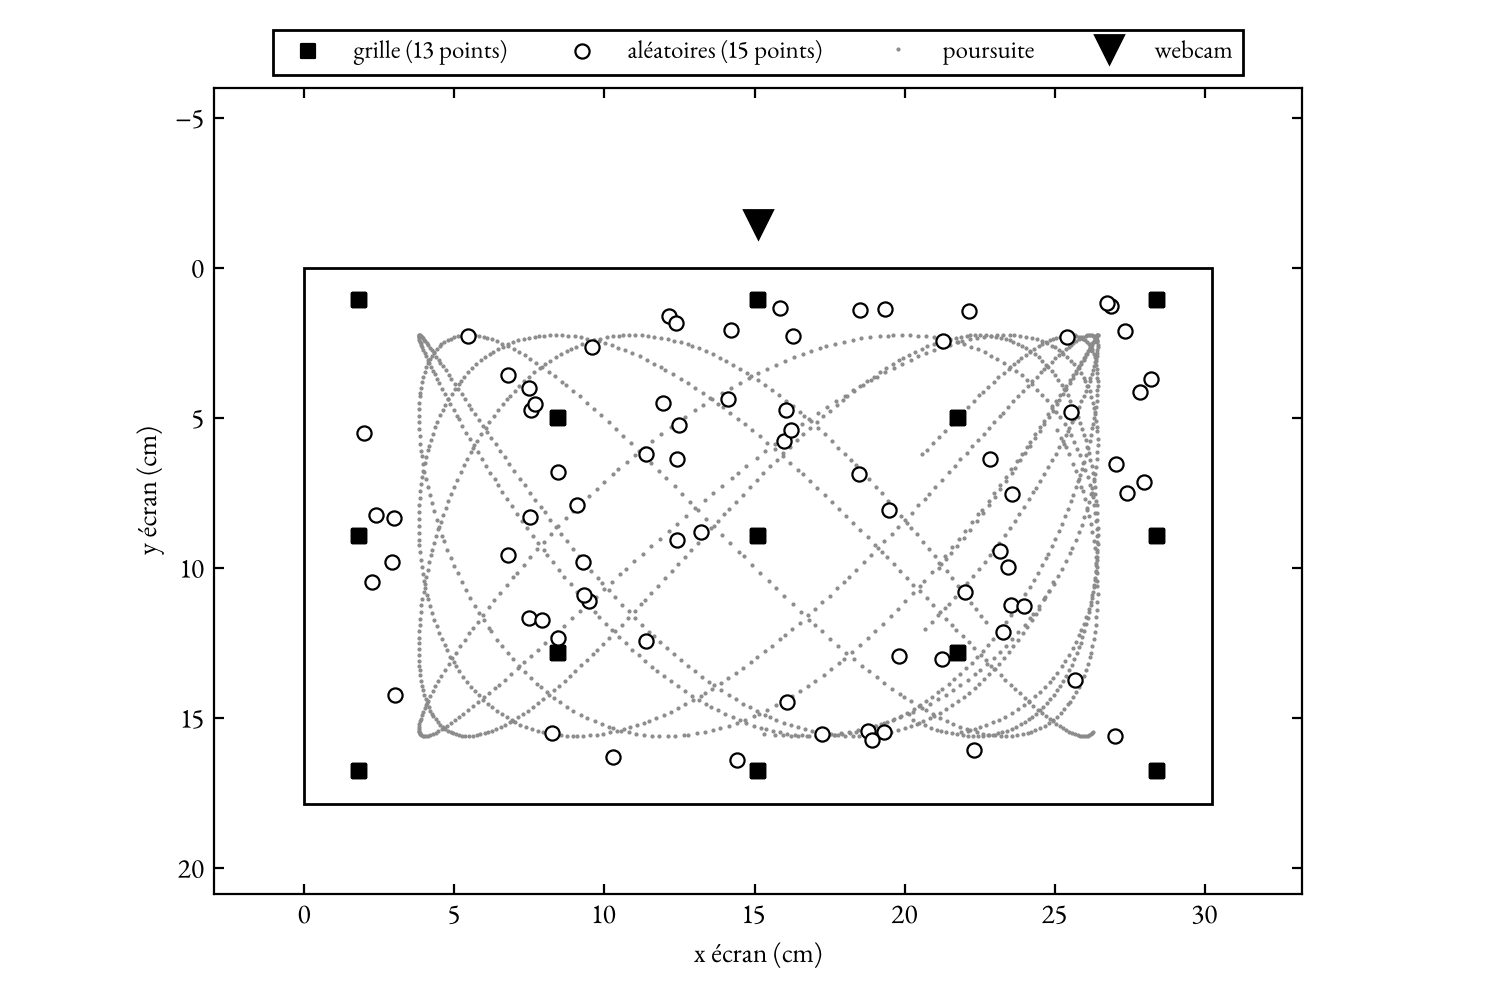
\includegraphics[width=0.72\linewidth]{fig01_protocole.png}
\caption{Cibles de la séance sur l'écran (30,2$\times$17,9~cm). Les points de grille occupent les mêmes positions à chaque tour.}\label{fig:protocole}
\end{figure}

L'horloge de la vidéo et celle de la page diffèrent d'un décalage inconnu $\tau$, que l'on retrouve grâce à deux flashs blancs émis par la page à des instants connus $[a_k,b_k]$. Soit $\ell_n$ la luminance moyenne du centre de l'image $n$, prise à l'instant $t_n$. On retire la tendance lente par un filtre médian de 31 images, puis on standardise de manière robuste :
\begin{equation}
z_n=\frac{\tilde\ell_n-\med(\tilde\ell)}{1{,}4826\,\MAD(\tilde\ell)},\qquad \tilde\ell_n=\ell_n-\med_{|m-n|\le15}\ell_m .
\end{equation}
Pour une loi normale $\mathcal N(\mu,\sigma^2)$, on a $\MAD=\sigma\,\Phi^{-1}(3/4)=0{,}6745\,\sigma$ (symétrie de la loi normale et définition de la médiane), d'où $\sigma=1{,}4826\,\MAD$, ce qui justifie le facteur. Le décalage retenu est
\begin{equation}
\hat\tau=\argmax_{\tau}\ \min_k\ \frac{1}{|I_k(\tau)|}\sum_{n\in I_k(\tau)} z_n,\qquad I_k(\tau)=\{n:\ a_k+\tau\le t_n<b_k+\tau\},
\end{equation}
cherché sur une grille de pas 1~ms. Le minimum sur $k$ exige que les deux flashs soient éclairés à la fois et élimine ainsi les maxima parasites qu'un seul flash laisserait passer ; on obtient $\hat\tau=193$~ms. L'œil, de son côté, met du temps à rejoindre une cible qui vient d'apparaître : environ 200~ms de latence, puis quelques corrections. On ne retient donc comme images de fixation que celles dont la cible est affichée depuis au moins 450~ms et pour encore au moins 50~ms, soit 3\,974 images sur 9\,283, et comme images de poursuite celles qui suivent de plus de 800~ms le début du mouvement, soit 1\,684 images. Le visage est détecté sur 9\,282 images sur 9\,283 ; toutes sont traitées, mais seules ces images, dont on sait ce que l'œil regarde, servent à mesurer l'erreur.

\section{Des yeux à la pupille}\label{sec:detect}

MediaPipe Face Landmarker \cite{kartynnik2019} détecte le visage dans chaque image et y ajuste un maillage de 478 points ; en mode vidéo, il suit le visage d'une image à l'autre, ce qui stabilise les points. Pour chaque œil, on retient les 16 points du contour des paupières et les 5 points de l'iris, un centre et quatre points du bord (figure~\ref{fig:detection}). Le rayon apparent $\rho$ est la plus grande des demi-étendues horizontale et verticale de ces quatre points : c'est le grand axe de l'ellipse du limbe, que la rotation de l'œil ne raccourcit pas (figure~\ref{fig:oeil}b).

\begin{figure}[!htbp]
\centering
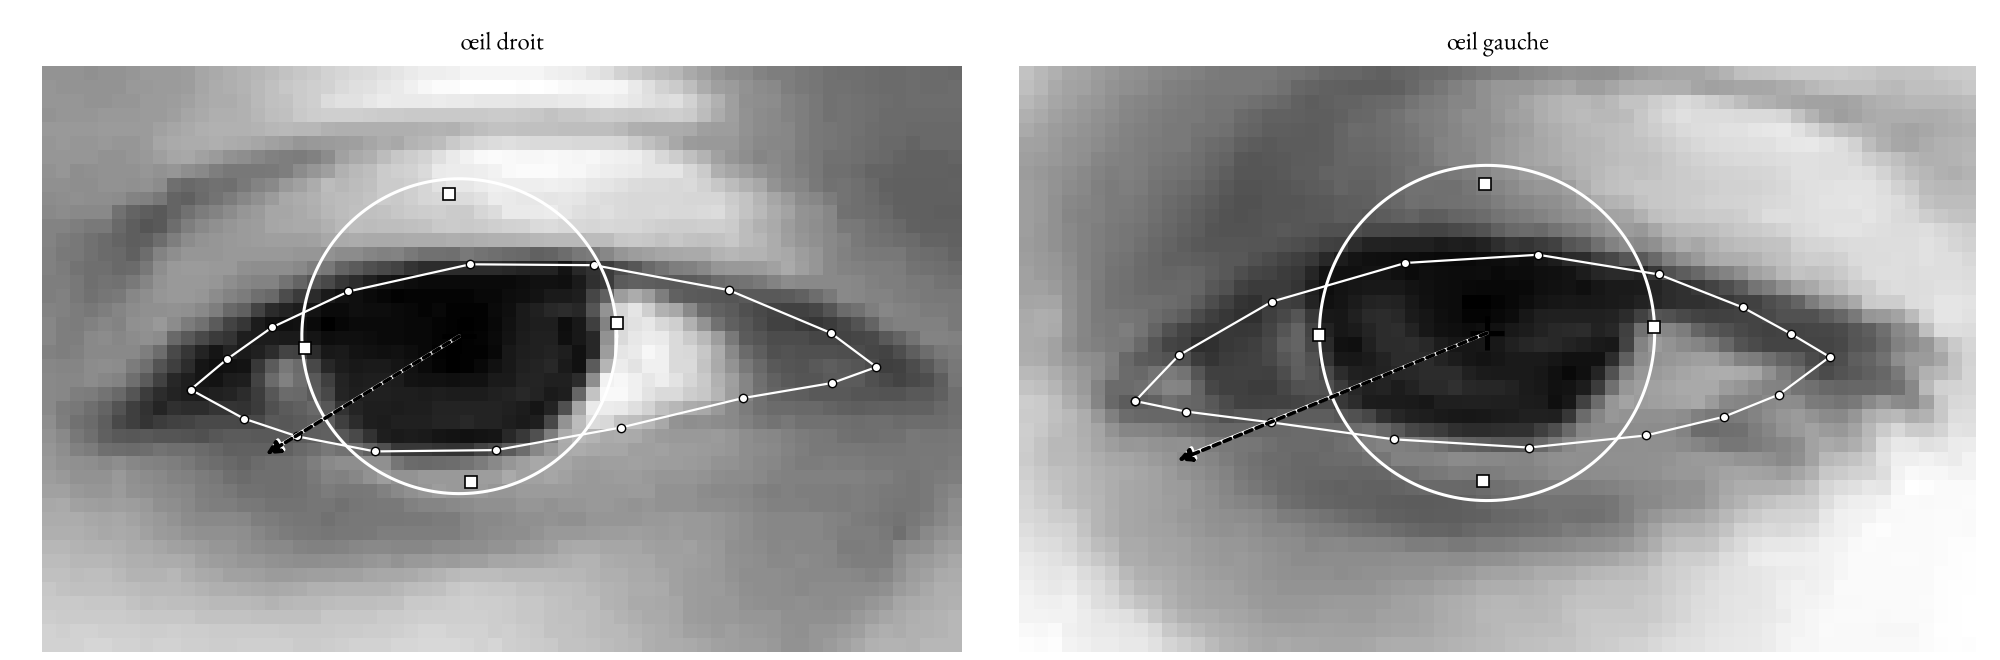
\includegraphics[width=\textwidth]{fig10_detection.png}
\caption{Détection sur une image de la séance (tour 1, fixation d'un point de grille). Ronds : contour des paupières ; carrés : bord du limbe ; cercle : limbe de rayon $\rho$ ; croix : centre du limbe $\vect p$, pris pour centre de la pupille. La flèche blanche est le vecteur regard estimé par un modèle qui n'a jamais vu cette cible, la flèche noire en tirets la direction vraie de l'œil vers la cible ; toutes deux sont les projections sur l'image des vecteurs 3D, issues de la pupille.}\label{fig:detection}
\end{figure}

C'est le centre de la pupille que l'on voudrait suivre, puisque c'est par elle que la lumière entre. On pourrait chercher à la segmenter, mais trois raisons font préférer le centre du limbe, frontière entre l'iris et le blanc de l'œil. Le contraste, d'abord : avec un iris brun et en lumière visible, la pupille se distingue à peine de l'iris, alors que le limbe est le contour le plus net de l'œil. La réfraction, ensuite : la pupille est vue à travers la cornée, sous la forme d'une image virtuelle agrandie d'environ 13\,\% et avancée d'environ 0,5~mm, dont la position apparente dépend de l'angle de vue, tandis que le limbe, au bord de la cornée, échappe presque entièrement à cette déformation. La concentricité, enfin : la pupille est centrée sur le limbe à quelques dixièmes de millimètre près, et un décentrement $\delta\approx0{,}2$~mm vu depuis le centre de rotation, à $d_L=10{,}4$~mm, produit un biais
\begin{equation}
\arcsin\frac{\delta}{d_L}\approx\frac{\delta}{d_L}=0{,}019~\text{rad}\approx1{,}1^\circ\qquad(\arcsin x\sim x\ \text{en }0),
\end{equation}
constant pour une personne donnée, que la direction de repos du modèle physique et l'ordonnée à l'origine de la calibration absorbent entièrement. Le centre du limbe est donc la meilleure estimation du centre de la pupille accessible à une webcam.

\section{Géométrie de la scène}\label{sec:geo}

On travaille dans le repère de la caméra : $x$ vers la droite de l'image, $y$ vers le haut, $z$ orienté de l'utilisateur vers la caméra. Le visage est donc en $z<0$ et un regard dirigé vers l'écran a une composante $g_z>0$. Une direction unitaire $\vect g$ est décrite par ses angles de Fick, lacet $\theta$ et tangage $\varphi$,
\begin{equation}
\theta=\operatorname{atan2}(g_x,g_z),\qquad \varphi=\arcsin g_y,\qquad
\vect g=(\cos\varphi\sin\theta,\ \sin\varphi,\ \cos\varphi\cos\theta)\T ,
\end{equation}
et l'on vérifie $\|\vect g\|^2=\cos^2\varphi(\sin^2\theta+\cos^2\theta)+\sin^2\varphi=1$ (identité $\cos^2+\sin^2=1$, deux fois). MediaPipe fournit pour chaque image une matrice de pose $\mathbf M=\begin{psmallmatrix}\mathbf R&\vect t\\0&1\end{psmallmatrix}$ qui envoie le visage canonique dans le repère caméra ; une direction $\vect g$ du repère caméra s'écrit donc $\mathbf R\T\vect g$ dans le repère de la tête ($\mathbf R$ orthogonale, donc $\mathbf R^{-1}=\mathbf R\T$).

La focale $f$ de la webcam est inconnue. Le modèle sténopé donne, pour un objet de taille $s$ vu de face à la distance $D$, une taille image $f\,s/D$ (théorème de Thalès). Or le rayon du limbe est la constante biométrique la plus stable du visage, $r_L=5{,}9\pm0{,}25$~mm. Si $\rho_n$ est le rayon apparent de l'iris en pixels et $D_n$ la distance de la tête fournie par la pose, alors $\rho_n=f\,r_L/D_n$ pour toute image, et l'on prend
\begin{equation}\label{eq:focal}
\hat f=\frac{\med_n(\rho_n D_n)}{r_L}=1\,012~\text{px},
\end{equation}
la médiane, dont le point de rupture est de 50\,\%, résistant aux images où l'iris est mal localisé. Avec cette focale, la projection sténopé $u-c_u=f\,X/D$, $v-c_v=-f\,Y/D$ s'inverse et place chaque œil en
\begin{equation}
\vect e=\Bigl(\frac{(u-c_u)D}{f},\ -\frac{(v-c_v)D}{f},\ -D\Bigr)\T ,
\end{equation}
où $(u,v)$ est le centre de l'iris dans l'image, $(c_u,c_v)$ le centre de l'image et $D$ la distance de la tête, lissée sur 15 images. On note $\vect e_L,\vect e_R$ les deux yeux et $\vect c=\tfrac12(\vect e_L+\vect e_R)$ l'œil cyclope, origine commune du regard binoculaire.

La webcam d'un portable est dans le cadre de l'écran ; on prend donc l'écran comme plan $z=0$. Un point de l'écran de coordonnées $(X_s,Y_s)$, en millimètres, $X_s$ vers la droite et $Y_s$ vers le bas tels que les voit l'utilisateur, et une webcam située en $(X_c,Y_c)$ sur ce même écran, donnent dans le repère caméra
\begin{equation}
\vect P=\bigl(-(X_s-X_c),\ -(Y_s-Y_c),\ 0\bigr)\T ,
\end{equation}
le premier signe venant de ce que la caméra fait face à l'utilisateur, dont la droite est la gauche de l'image. L'échelle est de 0,2~mm par pixel CSS sur cette machine. La webcam est au milieu du bord supérieur ; dans le repère de la page affichée, elle est en $(X_c,Y_c)=(151{,}2;\,-14{,}4)$~mm, l'ordonnée négative tenant compte de la barre du navigateur. Cette position est connue par construction, on la fixe au lieu de l'ajuster. Le rayon du regard $\vect c+s\,\vect g$, $s\ge0$, rencontre le plan $z=0$ lorsque $c_z+s\,g_z=0$, soit pour $s^\star=-c_z/g_z>0$ puisque $c_z<0$ et $g_z>0$, et le point regardé est
\begin{equation}\label{eq:hit}
\vect H=\vect c-\frac{c_z}{g_z}\,\vect g .
\end{equation}
L'erreur se mesure en distance sur l'écran, $\|\vect H_{xy}-\vect P_{xy}\|$, ou en angle, $\arccos(\vect g\cdot\vect u)$ avec $\vect u=(\vect P-\vect c)/\|\vect P-\vect c\|$ ; à 52~cm, un degré vaut $520\tan1^\circ\approx9{,}1$~mm au centre de l'écran.

\begin{figure}[!htbp]
\centering
\begin{tikzpicture}[x=0.235cm,y=0.235cm,>={Stealth[length=1.6mm]},font=\footnotesize]
\fill[black!4] (0,0) circle (11.96);
\fill[black!4] (5.3,0) circle (7.8);
\draw[line width=0.9pt] (29.57:11.96) arc (29.57:330.43:11.96);
\draw[line width=0.9pt] (5.3,0)++(-49.17:7.8) arc (-49.17:49.17:7.8);
\draw[black!45,densely dashed] (5.3,0)++(49.17:7.8) arc (49.17:310.83:7.8);
\draw[black!35] (7.4,0) ellipse (1.9 and 4.4);
\draw[line width=2.2pt] (10.4,1.8) -- (10.4,5.9);
\draw[line width=2.2pt] (10.4,-1.8) -- (10.4,-5.9);
\draw[thick] (-11.85,1.6) -- (-16,2.0);
\draw[thick] (-11.85,-1.6) -- (-16,-2.0);
\draw[black!50] (-16,0) -- (24,0);
\draw[->,densely dashed] (5.3,0) -- ++(5:19.5) node[right] {axe visuel};
\draw[->,line width=1.3pt] (10.4,0) -- (23,0) node[right] {$\bm o$};
\node[align=left,anchor=north west] at (16.2,-0.6) {axe optique,\\normale au plan\\du limbe};
\draw (13.4,0) arc (0:5:8.1);
\node at (14.4,1.15) {$\theta_\kappa$};
\draw (10.4,0) -- (10.4,0.9) -- (11.3,0.9) -- (11.3,0);
\draw (5.3,0) -- node[above left=-2pt] {$r_c$} (10.4,5.9);
\draw (0,0) -- node[below left=-1pt] {$R_e$} (10.4,-5.9);
\draw[dotted] (10.4,5.9) -- (18.9,5.9);
\draw[<->] (18.2,0.15) -- node[right] {$r_L$} (18.2,5.75);
\draw[dotted] (0,-0.5) -- (0,-15.2);
\draw[dotted] (10.4,-6.4) -- (10.4,-15.2);
\draw[dotted] (5.3,-0.5) -- (5.3,-12.6);
\draw[<->] (0,-14.6) -- node[below] {$d_L=10{,}4$ mm} (10.4,-14.6);
\draw[<->] (0,-12) -- node[below] {$5{,}3$} (5.3,-12);
\draw[<->] (5.3,-12) -- node[below] {$d_{ci}$} (10.4,-12);
\fill (0,0) circle (0.35) node[above left] {$\bm c_e$};
\fill (5.3,0) circle (0.3) node[above left=-1pt] {$\bm O_c$};
\fill (10.4,0) circle (0.3) node[below right=-1pt] {$\bm L$};
\node[align=center] at (-5,6.5) {globe\\$R_e\approx12$ mm};
\node at (15.6,-7.6) {cornée, $r_c=7{,}8$ mm};
\node at (4.2,-8.6) {cristallin};
\node[align=left] at (19,9.2) {iris : cercle du limbe};
\draw[black!60] (16.1,8.6) -- (10.6,4.6);
\node[align=center] at (-16.5,-4.2) {nerf\\optique};
\node at (-16,12.5) {\textsc{(a)}};
\end{tikzpicture}

\vspace{4mm}

\begin{tikzpicture}[x=0.235cm,y=0.235cm,>={Stealth[length=1.6mm]},font=\footnotesize]
\def\th{28}
\fill[black!4] (0,0) circle (11.96);
\fill[black!4] (\th:5.3) circle (7.8);
\draw[line width=0.9pt] (\th+29.57:11.96) arc (\th+29.57:\th+330.43:11.96);
\draw[line width=0.9pt] (\th:5.3)++(\th-49.17:7.8) arc (\th-49.17:\th+49.17:7.8);
\draw[line width=2.2pt] ($(\th:10.4)+(\th+90:5.9)$) -- ($(\th:10.4)+(\th+90:1.8)$);
\draw[line width=2.2pt] ($(\th:10.4)+(\th-90:1.8)$) -- ($(\th:10.4)+(\th-90:5.9)$);
\draw[black!50] (-13,0) -- (31,0);
\draw[->,line width=1.3pt] (\th:10.4) -- (\th:22) node[above] {$\bm o$};
\draw (\th:10.4) -- ++(\th+90:0.9) -- ++(\th:0.9) -- ++(\th-90:0.9);
\draw (6,0) arc (0:\th:6) node[midway,right] {$\theta$};
\fill (0,0) circle (0.35) node[below left] {$\bm c_e$};
\fill (\th:10.4) circle (0.3) node[below right=-1pt] {$\bm L$};
\draw[line width=1.1pt] (27,-13) -- (27,13) node[above] {plan image};
\node[align=center,anchor=north] at (27,-13.4) {projection parallèle\\d'échelle $\kappa=f/D$};
\draw[densely dotted] (\th:10.4) -- (27,{10.4*sin(\th)});
\draw[densely dotted] ($(\th:10.4)+(\th+90:5.9)$) -- (27,{10.4*sin(\th)+5.9*cos(\th)});
\draw[densely dotted] ($(\th:10.4)+(\th-90:5.9)$) -- (27,{10.4*sin(\th)-5.9*cos(\th)});
\fill (27,0) circle (0.3) node[right] {$\bm q$};
\fill (27,{10.4*sin(\th)}) circle (0.3) node[right] {$\bm p$};
\draw[<->] (24.6,0.2) -- node[left,align=right] {$\kappa\,d_L\sin\theta$\\$=\gamma\rho\sin\theta$} (24.6,{10.4*sin(\th)-0.2});
\draw[decorate,decoration={brace,amplitude=4pt}] (28.6,{10.4*sin(\th)+5.9*cos(\th)}) -- (28.6,{10.4*sin(\th)-5.9*cos(\th)}) node[midway,right=4pt,align=left] {$2\kappa r_L\cos\theta$\\(petit axe de\\l'ellipse)};
\draw[->] (31,0) -- (33.5,0) node[below] {$z$};
\node at (-14,12.5) {\textsc{(b)}};
\end{tikzpicture}

\caption{Géométrie de l'œil, à l'échelle. \textsc{(a)}~Coupe horizontale : globe et cornée sont deux sphères dont l'intersection est le limbe, cercle de rayon $r_L$ qui borde l'iris ; le regard (axe optique $\vect o$) est la normale à ce cercle, issue du centre de rotation $\vect c_e$. L'axe visuel, qui passe par la fovéa, en diffère d'un angle $\theta_\kappa\approx5^\circ$, absorbé par la direction de repos. \textsc{(b)}~Observation : tourné d'un angle $\theta$, le centre du limbe se projette à $\kappa d_L\sin\theta$ de la projection du centre de rotation, tandis que le cercle devient une ellipse dont seul le petit axe se raccourcit.}\label{fig:oeil}
\end{figure}

Le globe est une sphère de centre $\vect c_e$ ; la cornée en est une seconde, de rayon $r_c=7{,}8$~mm, dont le centre est à 5,3~mm de $\vect c_e$ le long de l'axe optique $\vect o$. Leur intersection est le limbe, un cercle de rayon $r_L=5{,}9$~mm dont $\vect o$ est la normale issue du centre (figure~\ref{fig:oeil}a) : lire la direction du regard, c'est lire l'orientation de ce cercle. Son plan est à la distance
\begin{equation}
d_{ci}=\sqrt{r_c^2-r_L^2}=\sqrt{7{,}8^2-5{,}9^2}=\sqrt{60{,}84-34{,}81}=\sqrt{26{,}03}=5{,}10~\text{mm}
\end{equation}
du centre cornéen (théorème de Pythagore dans le triangle formé par le centre cornéen, le centre du limbe et un point du limbe). Le centre du limbe est donc à $d_L=5{,}3+5{,}10=10{,}40$~mm du centre de rotation, et le rapport utile vaut
\begin{equation}
\gamma=\frac{d_L}{r_L}=\frac{10{,}40}{5{,}9}=1{,}763 .
\end{equation}
Le rayon du globe s'en déduit, $R_e=\sqrt{r_L^2+d_L^2}=\sqrt{34{,}81+108{,}16}=11{,}96$~mm (Pythagore à nouveau), en accord avec la valeur anatomique de 12~mm, ce qui confirme la cohérence des constantes.

Soit $\vect p$ la projection du centre du limbe et $\vect q$ celle du centre de rotation. Le visage étant petit devant sa distance, on adopte la projection perspective faible d'échelle $\kappa=f/D$ pixels par millimètre. Comme $\vect L=\vect c_e+d_L\vect o$, la linéarité de cette projection donne $\vect p-\vect q=\kappa\,d_L\,(o_x,\,-o_y)\T$, le signe de $y$ venant de l'axe image descendant. Le rayon apparent de l'iris vaut $\rho=\kappa r_L$, donc $\kappa\,d_L=\gamma\rho$, et
\begin{equation}\label{eq:observation}
(o_x,\,-o_y)=\frac{\vect p-\vect q}{\gamma\,\rho},\qquad o_z=\sqrt{1-o_x^2-o_y^2}
\end{equation}
($\|\vect o\|=1$ et $o_z>0$ pour un œil tourné vers la caméra). Ni $f$ ni $D$ n'apparaissent : seul le rayon de l'iris fixe l'échelle, à condition de le lire sur le grand axe de l'ellipse, $\kappa r_L$, et non sur le petit, $\kappa r_L\cos\theta$. Pour limiter le bruit, $\rho$ est prédit par $\rho_n=k/D_n$ avec $k=\med(\rho_nD_n)$, la quantité même qui a donné la focale. Le centre de rotation, lui, n'est pas visible. On le place à une profondeur $b$ derrière le milieu $\vect m$ des coins de l'œil, le long de la normale du visage ; la troisième colonne $\vect r_3$ de $\mathbf R$ est cette normale, dont la projection image, de sens opposé, est $(-r_{13},\,r_{23})$, d'où
\begin{equation}
\vect q=\vect m+\frac{b\,\rho}{r_L}\,(-r_{13},\ r_{23})\T,
\end{equation}
où $\rho/r_L=\kappa$ convertit les millimètres en pixels.

Il reste à corriger ce que les points de MediaPipe ont d'imparfait. La paupière supérieure suit le globe et entraîne le centre d'iris vers le haut ou le bas ; on corrige la composante verticale de \eqref{eq:observation} par $-\lambda_p(a-\bar a)$, où $a$ est l'ouverture palpébrale normalisée par la largeur de l'œil et $\bar a$ sa médiane. La direction obtenue est ramenée dans le repère de la tête, tournée pour qu'une direction de repos $(\theta_0,\varphi_0)$ propre à chaque œil devienne l'axe $z$, et ses angles de Fick sont multipliés par des gains $(G_x,G_y)$. Ces huit paramètres, deux directions de repos, deux gains, $b$ et $\lambda_p$, sont ajustés en minimisant la somme sur les deux yeux des écarts angulaires $r_i$ entre direction prédite et direction vraie $\vect P-\vect e$. Pour résister aux images aberrantes, on emploie la perte soft-$L_1$, $\rho_c(r)=2c^2\bigl(\sqrt{1+(r/c)^2}-1\bigr)$ avec $c=2^\circ$, par moindres carrés repondérés. Sa dérivée est $\psi_c(r)=\rho_c'(r)/2=r/\sqrt{1+(r/c)^2}$ (dérivée d'une composée), donc le poids vaut
\begin{equation}
w(r)=\frac{\psi_c(r)}{r}=\Bigl(1+\frac{r^2}{c^2}\Bigr)^{-1/2},
\end{equation}
et chaque résidu est multiplié par $\sqrt{w}=(1+r^2/c^2)^{-1/4}$, puisque $(\sqrt w\,r)^2=w\,r^2$ ; quatre itérations de Levenberg--Marquardt suffisent.

\begin{table}[!htbp]
\centering\small
\begin{tabular}{@{}lr@{\qquad}lr@{}}
\toprule
Paramètre & Valeur & Paramètre & Valeur\\
\midrule
repos œil gauche $(\theta_0,\varphi_0)$ & $(-9{,}8^\circ,\ 10{,}7^\circ)$ & gain horizontal $G_x$ & 1,62\\
repos œil droit $(\theta_0,\varphi_0)$ & $(10{,}1^\circ,\ 10{,}5^\circ)$ & gain vertical $G_y$ & 3,07\\
profondeur du centre $b$ & 8,7~mm & gain de paupière $\lambda_p$ & 0,42\\
webcam $(X_c,Y_c)$, fixée & $(151{,}2;\ -14{,}4)$~mm & focale $\hat f$ & 1\,012~px\\
\bottomrule
\end{tabular}
\caption{Paramètres du modèle physique ajustés sur toute la séance.}\label{tab:physique}
\end{table}

Les valeurs du tableau~\ref{tab:physique} disent à elles seules la faiblesse de la géométrie. Le gain vertical de 3,07 signifie que MediaPipe écrase les mouvements verticaux de l'iris d'un facteur trois, si bien que tout bruit vertical est triplé à la sortie. Quant aux directions de repos, voisines de $\pm10^\circ$ en lacet et de $10^\circ$ en tangage, elles ne mesurent pas seulement l'angle $\theta_\kappa$ entre axe optique et axe visuel : elles absorbent le décalage vertical entre le milieu des coins de l'œil et le centre du globe, ainsi que les biais propres aux points de MediaPipe. La flèche brute $\vect q\to\vect p$ n'est donc pas le regard ; il faut lui appliquer la rotation de repos, et c'est le regard ainsi corrigé, puis calibré, que montre la figure~\ref{fig:detection}.

\section{Apparence : réseaux pré-entraînés}\label{sec:app}

Les réseaux de regard sont entraînés sur des images normalisées \cite{zhang2018revisiting}, prises par une caméra virtuelle placée face au visage, à distance fixe $d_n$, sans roulis. Si $\vect h$ est le centre du visage en 3D et $\vect x_h$ l'axe horizontal de la tête, cette caméra a pour repère
\begin{equation}
\vect z_n=\frac{\vect h}{\|\vect h\|},\qquad
\vect y_n=\frac{\vect z_n\times\vect x_h}{\|\vect z_n\times\vect x_h\|},\qquad
\vect x_n=\vect y_n\times\vect z_n,\qquad
\mathbf R_n=\begin{pmatrix}\vect x_n\T\\ \vect y_n\T\\ \vect z_n\T\end{pmatrix}.
\end{equation}
Les trois vecteurs sont unitaires et deux à deux orthogonaux ($\vect y_n\perp\vect z_n$ et $\vect x_n\perp\vect y_n,\vect z_n$ par construction du produit vectoriel, $\|\vect x_n\|=\|\vect y_n\|\|\vect z_n\|\sin\frac\pi2=1$), donc $\mathbf R_n$ est une rotation. Avec $\mathbf S=\operatorname{diag}(1,1,d_n/\|\vect h\|)$ et les matrices intrinsèques $\mathbf C$, réelle, et $\mathbf C_n$, virtuelle, l'image est déformée par l'homographie $\mathbf W=\mathbf C_n\mathbf S\mathbf R_n\mathbf C^{-1}$. Le regard, lui, n'est transformé que par la rotation, $\vect g_n=\mathbf R_n\vect g$, car $\mathbf S$ rapproche la caméra sans changer la direction vers laquelle l'œil est tourné ; la prédiction du réseau revient donc au repère caméra par $\vect g=\mathbf R_n\T\vect g_n$, au changement de repère d'OpenCV près, $(x,y,z)\mapsto(x,-y,-z)$, rotation d'angle $\pi$ autour de $x$. C'est ici que la géométrie sert l'apparence : la normalisation exige les intrinsèques de la caméra, que seule la focale \eqref{eq:focal} nous donne.

Deux réseaux sont mis à contribution, avec les poids publiés par la bibliothèque \texttt{ptgaze} \cite{hysts}. MPIIFaceGaze \cite{zhang2017mpiifacegaze} a été entraîné sur quinze personnes filmées au quotidien par la webcam de leur portable : il a vu exactement notre type d'images. ETH-XGaze \cite{zhang2020eth} a vu 110 personnes, plus d'un million d'images et des postures de tête extrêmes ; on en garde la direction prédite et l'embedding de dimension 512 qui précède la sortie. Sans calibration, ces réseaux font respectivement 4,81 et 4,64~cm d'erreur médiane sur nos images de fixation : ils sont robustes, mais pas exacts pour cette personne.

\section{Calibration en deux étages}\label{sec:cal}

Notons $\vect a_n\in\R^2$ les angles de Fick prédits par MPIIFaceGaze dans le repère caméra et $\vect y_n\in\R^2$ les angles vrais, de $\vect c_n$ vers la cible $\vect P_n$. Le premier étage cherche $\mathbf W\in\R^{3\times2}$ tel que $\vect y_n\approx(\vect a_n\T,1)\,\mathbf W$. Avec $\mathbf A\in\R^{N\times3}$ la matrice des lignes $(\vect a_n\T,1)$, $\mathbf Y\in\R^{N\times2}$ celle des $\vect y_n\T$, et $\mathbf D=\operatorname{diag}(1,1,0)$ qui épargne l'ordonnée à l'origine,
\begin{align}
J(\mathbf W)&=\|\mathbf A\mathbf W-\mathbf Y\|_F^2+\lambda\|\mathbf D\mathbf W\|_F^2,\\
\nabla J(\mathbf W)&=2\mathbf A\T(\mathbf A\mathbf W-\mathbf Y)+2\lambda\mathbf D\T\mathbf D\mathbf W
\quad(\text{dérivée de }\|\mathbf X\|_F^2=\operatorname{tr}\mathbf X\T\mathbf X)\\
&=2\bigl[(\mathbf A\T\mathbf A+\lambda\mathbf D)\mathbf W-\mathbf A\T\mathbf Y\bigr]\quad(\mathbf D\T\mathbf D=\mathbf D,\ \text{projecteur}),
\end{align}
et $J$ étant convexe, somme de formes quadratiques positives, son minimum annule le gradient :
\begin{equation}
\hat{\mathbf W}=(\mathbf A\T\mathbf A+\lambda\mathbf D)^{-1}\mathbf A\T\mathbf Y,\qquad\lambda=10^{-3}N .
\end{equation}
Une application affine des angles a une propriété précieuse : elle est définie et raisonnable partout, y compris pour une posture de tête que la calibration n'a pas vue.

Le résidu $\vect r_n=\vect y_n-(\vect a_n\T,1)\hat{\mathbf W}$ contient le biais fin, propre à la personne. On le prédit à partir d'un vecteur $\vect x_n\in\R^{142}$ qui rassemble tout ce que la géométrie et l'apparence savent de l'œil. Les 21 points de chaque œil y figurent, exprimés dans le repère de ses propres coins, origine au milieu des coins, axe $x$ vers le coin opposé et échelle égale à la largeur de l'œil, repère qui efface la distance, la position dans l'image et le roulis de la tête. S'y ajoutent les 14 coefficients MediaPipe qui décrivent l'œil (clignement, regard vers le haut, le bas, l'intérieur, l'extérieur, plissement, écarquillement), les angles des deux réseaux dans le repère de la tête, et l'embedding d'ETH-XGaze réduit à 16 composantes principales. S'y ajoutent enfin les pixels des deux yeux : chaque œil est recadré par la similitude qui envoie ses deux coins sur deux points fixes d'une imagette de $64\times32$ pixels, chaque imagette est centrée-réduite, et les deux sont réduites ensemble à 24 composantes principales. Les points de MediaPipe résument l'œil en 21 positions précises au pixel près ; or un pixel de déplacement de la pupille vaut plusieurs degrés à 52~cm. Les imagettes rendent à la régression ce que les points ont perdu : la forme exacte du limbe, la part d'iris couverte par la paupière, le reflet.

Les variables étant centrées-réduites, on cherche $h$ dans l'espace de Hilbert à noyau reproduisant $\mathcal H$ du noyau gaussien $k(\vect x,\vect x')=\exp(-\gamma\|\vect x-\vect x'\|^2)$, avec $\gamma=0{,}5/142$, qui minimise
\begin{equation}
\sum_{n=1}^N\|\vect r_n-h(\vect x_n)\|^2+\alpha\|h\|_{\mathcal H}^2,\qquad\alpha=0{,}1 .
\end{equation}
Par le théorème du représentant \cite{scholkopf2001representer}, la solution s'écrit $\hat h=\sum_i\vect\beta_i\T k(\vect x_i,\cdot)$. Si $\mathbf B\in\R^{N\times2}$ est la matrice des $\vect\beta_i\T$, $\mathbf K=(k(\vect x_i,\vect x_j))_{ij}$ et $\mathbf E$ la matrice des résidus,
\begin{align}
J(\mathbf B)&=\|\mathbf E-\mathbf K\mathbf B\|_F^2+\alpha\operatorname{tr}(\mathbf B\T\mathbf K\mathbf B)\quad(\langle k(\vect x_i,\cdot),k(\vect x_j,\cdot)\rangle_{\mathcal H}=K_{ij}),\\
\nabla J(\mathbf B)&=-2\mathbf K(\mathbf E-\mathbf K\mathbf B)+2\alpha\mathbf K\mathbf B\quad(\mathbf K\text{ symétrique})\\
&=2\mathbf K\bigl[(\mathbf K+\alpha\mathbf I)\mathbf B-\mathbf E\bigr].
\end{align}
$\mathbf K$ est semi-définie positive, matrice de Gram d'un noyau défini positif, et $\alpha>0$ ; $\mathbf K+\alpha\mathbf I$ est donc définie positive et inversible, et
\begin{equation}
\hat{\mathbf B}=(\mathbf K+\alpha\mathbf I)^{-1}\mathbf E
\end{equation}
annule le gradient d'une fonction convexe, c'en est le minimum. La prédiction finale est $\hat{\vect y}(\vect x)=(\vect a\T,1)\hat{\mathbf W}+\sum_i\hat{\vect\beta}_i\,k(\vect x_i,\vect x)$.

Cette structure explique pourquoi le modèle dégrade gracieusement. Soit $\vect x$ une entrée éloignée de toutes les données de calibration, $\min_i\|\vect x-\vect x_i\|\ge\delta$. Alors
\begin{equation}\label{eq:extrapolation}
\Bigl\|\sum_i\hat{\vect\beta}_i\,k(\vect x_i,\vect x)\Bigr\|\le\sum_i\|\hat{\vect\beta}_i\|\,e^{-\gamma\|\vect x-\vect x_i\|^2}\le e^{-\gamma\delta^2}\sum_i\|\hat{\vect\beta}_i\|\ \xrightarrow[\delta\to\infty]{}\ 0
\end{equation}
(inégalité triangulaire, puis décroissance de $u\mapsto e^{-\gamma u}$). Loin de la zone calibrée, la correction s'éteint d'elle-même et le modèle retombe sur l'étage linéaire, qui extrapole. Les mesures le confirment : sur une posture jamais vue, le modèle complet (2,68~cm) fait jeu égal avec l'étage linéaire (2,65~cm), alors qu'un modèle appris de bout en bout sur nos seules données, sans cette structure, s'effondre. Au début d'une nouvelle séance, enfin, on peut faire regarder quelques points et corriger les prédictions par une application affine $\hat{\vect y}\mapsto\hat{\vect y}+(\hat{\vect y}\T,1)\mathbf C$, obtenue comme au premier étage,
\begin{equation}
\hat{\mathbf C}=(\mathbf B_r\T\mathbf B_r+\mu N_r\mathbf D)^{-1}\mathbf B_r\T(\mathbf Y_r-\hat{\mathbf Y}),\qquad\mu=0{,}05 ,
\end{equation}
où $\mathbf B_r$ rassemble les lignes $(\hat{\vect y}_n\T,1)$ des $N_r$ points regardés et $\mathbf Y_r$ leurs angles vrais.

\section{Protocole d'évaluation}\label{sec:eval}

On ne teste jamais sur une image qui a servi à l'ajustement, ni sur une image voisine d'une image d'ajustement, et l'on pose trois questions distinctes. La première, celle des cibles jamais vues, est traitée par une validation croisée en cinq plis groupés par cible : toutes les images d'une même cible tombent dans le même pli, si bien que les postures sont toutes connues mais que les positions testées ne l'ont jamais été. La deuxième, celle des postures jamais vues, retire un tour entier, ajuste sur les quatre autres, teste sur le tour retiré et répète l'opération pour chaque tour ; on rapporte la moyenne des cinq médianes. La troisième reprend la deuxième en autorisant la recalibration rapide sur les cinq premiers points de grille du tour retiré, testés à part. Chaque pli refait tout l'ajustement, modèle physique, étage linéaire, analyses en composantes principales et régression à noyau.

\section{Résultats}\label{sec:results}

\begin{table}[!htbp]
\centering\footnotesize
\begin{tabular}{@{}lccc@{}}
\toprule
& Géométrie & Réseau + linéaire & Modèle complet\\
\midrule
Cibles jamais vues, médiane & 4,02~cm (4,28°) & 2,15~cm (2,28°) & 0,83~cm (0,88°)\\
Cibles jamais vues, p90 & 7,45~cm & 5,11~cm & 2,08~cm\\
Posture jamais vue & 5,52~cm & 2,65~cm & 2,68~cm\\
Posture jamais vue + 5 points & 3,04~cm & 2,05~cm & 2,18~cm\\
\midrule
\multicolumn{4}{@{}l}{Sans calibration : MPIIFaceGaze 4,81~cm ; ETH-XGaze 4,64~cm.}\\
\bottomrule
\end{tabular}
\caption{Erreur sur l'écran, médiane par image, sur 3\,974 images de fixation (posture jamais vue : moyenne des médianes des cinq tours).}\label{tab:resultats}
\end{table}

Le tableau~\ref{tab:resultats} montre que chaque brique apporte sa part. Le réseau calibré linéairement divise presque par deux l'erreur de la géométrie seule, et la correction à noyau la divise encore par 2,6 ; au total, le modèle complet est 4,8 fois plus précis que la géométrie seule et 5,6 fois plus précis que le meilleur réseau public brut. Le gain ne se limite pas à la médiane : 90\,\% des images du modèle complet tombent à moins de 2,1~cm de la cible (figure~\ref{fig:cdf}), et les erreurs horizontale et verticale, dont la géométrie seule montre les queues larges, surtout en vertical où se lit le gain $G_y$, sont resserrées et centrées sur zéro (figure~\ref{fig:ecarts}). Carte à l'appui (figure~\ref{fig:carte}), les grosses erreurs de la géométrie se concentrent sur les bords et dans les coins, là où l'œil tourne le plus et où la paupière couvre le plus d'iris.

\begin{figure}[!htbp]
\centering
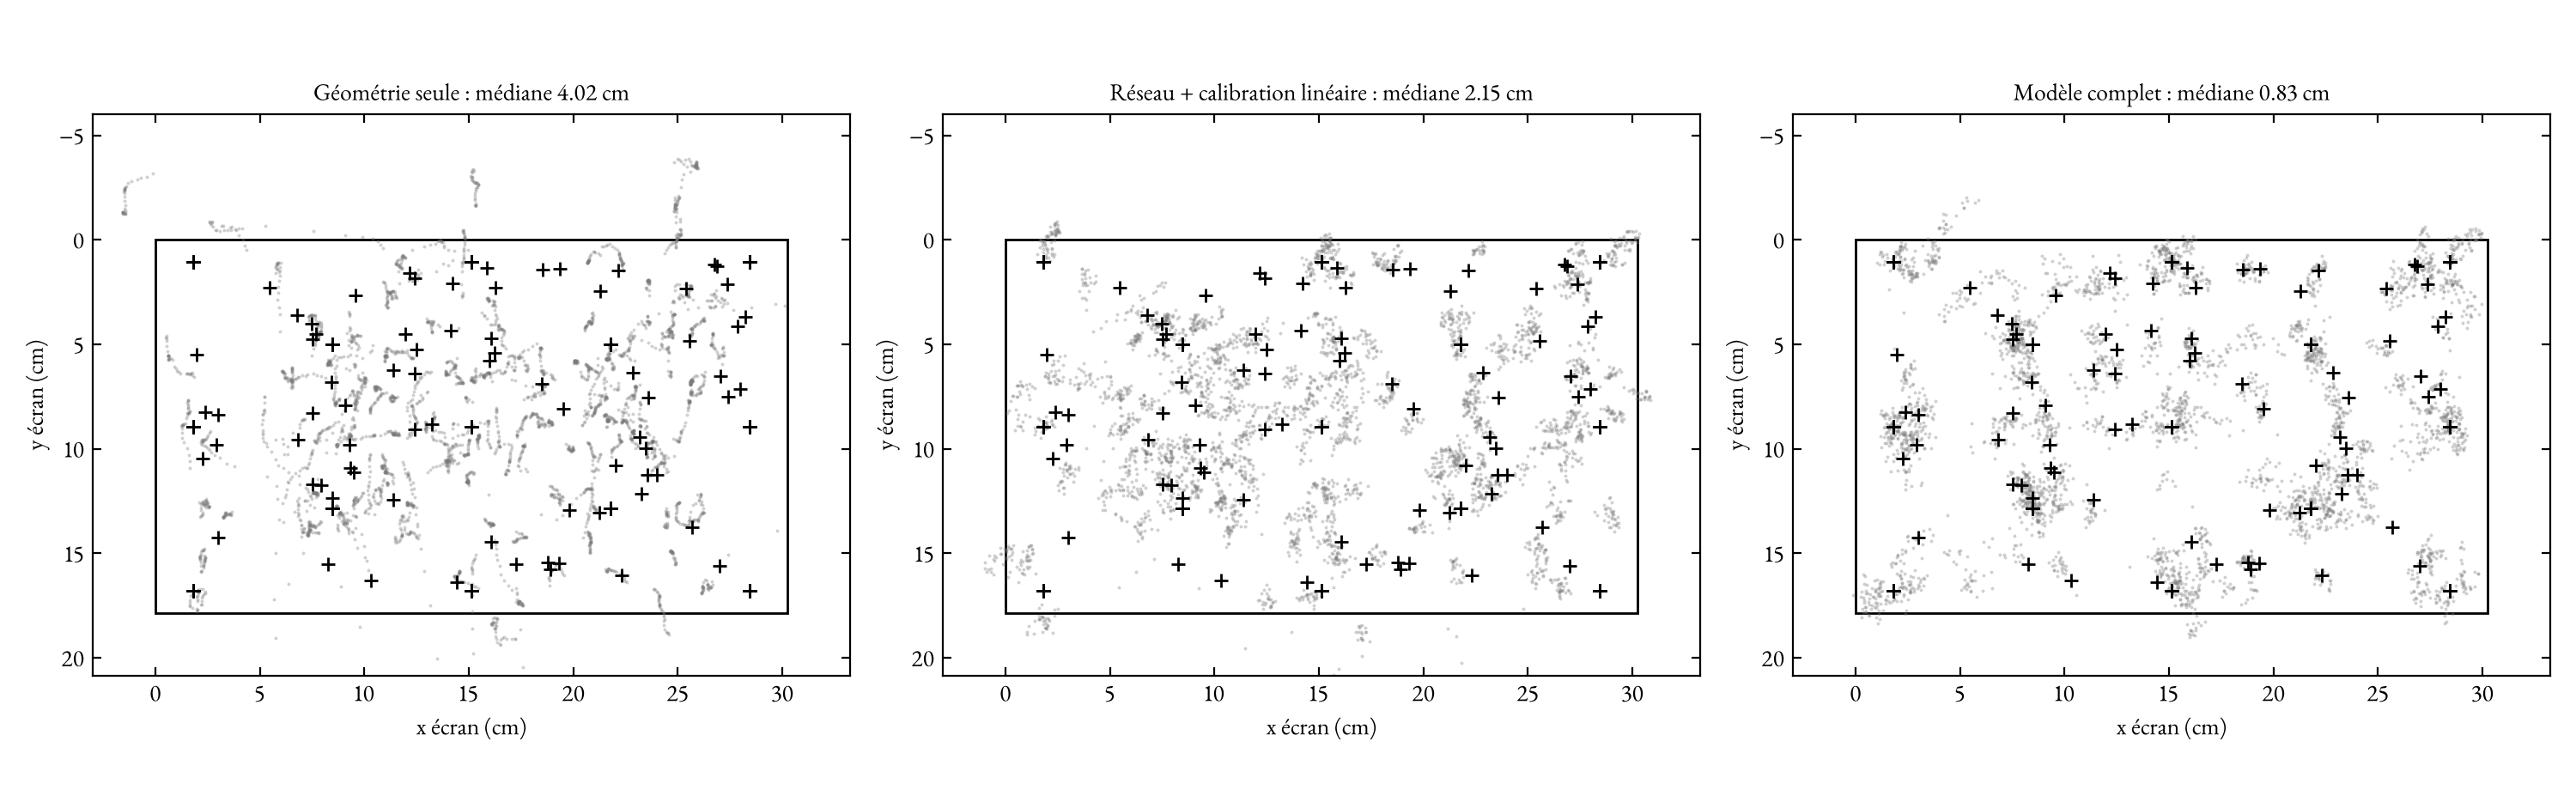
\includegraphics[width=\linewidth]{fig03_cibles_jamais_vues.png}
\caption{Cibles jamais vues : chaque point est une image de fixation, chaque croix une cible.}\label{fig:scatter}
\end{figure}

\begin{figure}[!htbp]
\centering
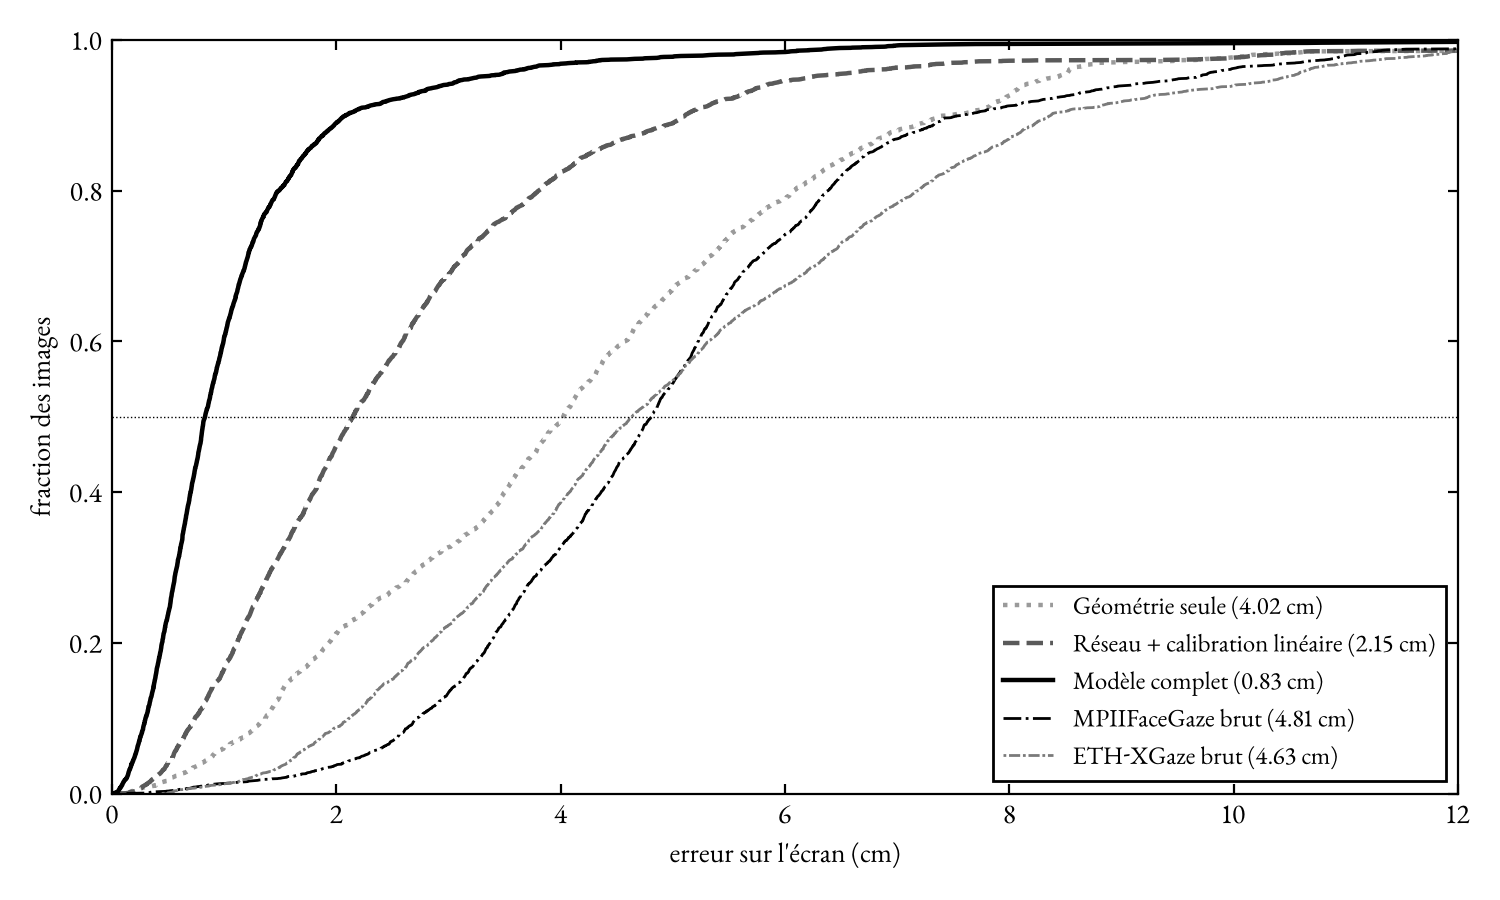
\includegraphics[width=0.75\linewidth]{fig04_repartition_erreurs.png}
\caption{Fonction de répartition de l'erreur sur l'écran (cibles jamais vues). Entre parenthèses, la médiane.}\label{fig:cdf}
\end{figure}

L'erreur par image mêle cependant deux choses qu'il faut séparer : un bruit d'une image à l'autre et un biais propre à chaque fixation. Le bruit se mesure par la dispersion des prédictions autour de leur médiane pendant une fixation, 0,39~cm. Le biais se mesure par l'écart entre cette médiane et la cible, 0,66~cm sur les 140 fixations (p90 1,70~cm) ; c'est ce second chiffre qui dit où la personne regarde. Il contient d'ailleurs l'erreur de la personne elle-même, car un œil qui fixe un point s'en écarte typiquement de 0,3 à $0{,}5^\circ$, soit 0,3 à 0,45~cm à cette distance. Sur nos fixations, le biais d'un même point de grille varie d'un tour à l'autre davantage qu'il ne se répète, 0,90~cm de variation contre 0,62~cm de partie commune : une partie de l'erreur restante vient de la posture et de la vérité terrain plutôt que d'un défaut fixe du modèle.

\begin{figure}[!htbp]
\centering
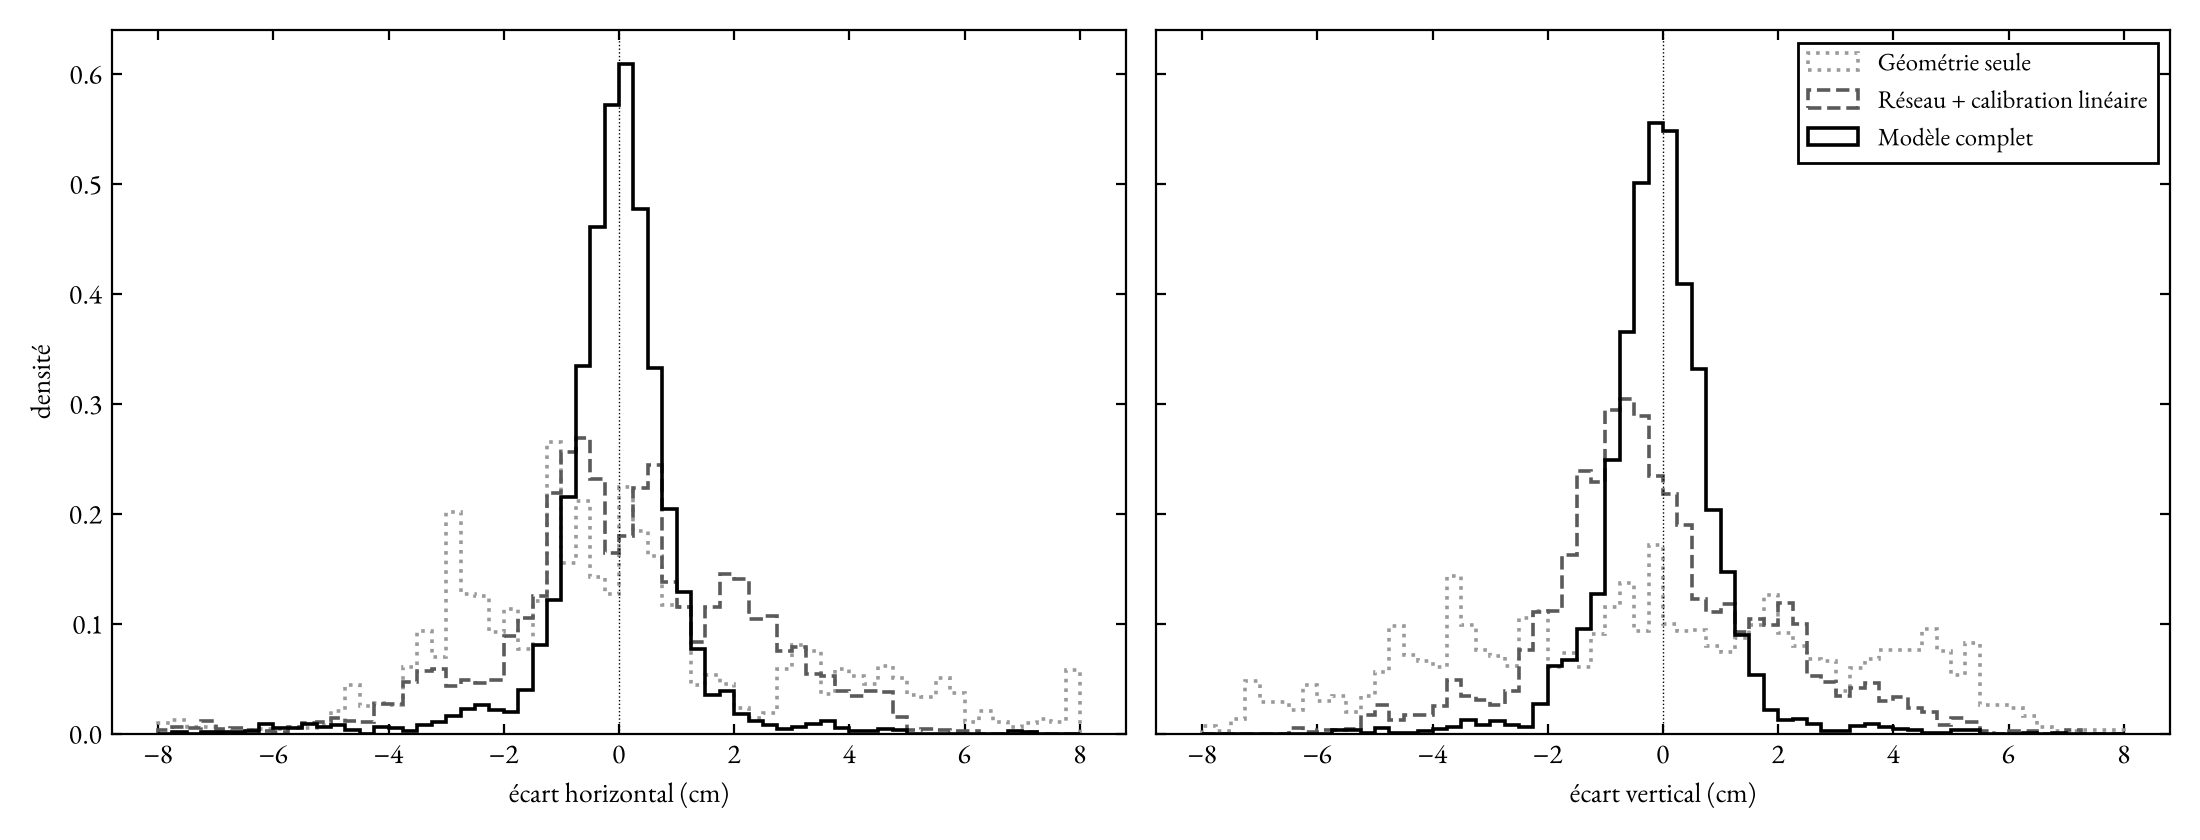
\includegraphics[width=0.95\linewidth]{fig07_ecarts_xy.png}
\caption{Écart signé entre point estimé et cible (cibles jamais vues).}\label{fig:ecarts}
\end{figure}

\begin{figure}[!htbp]
\centering
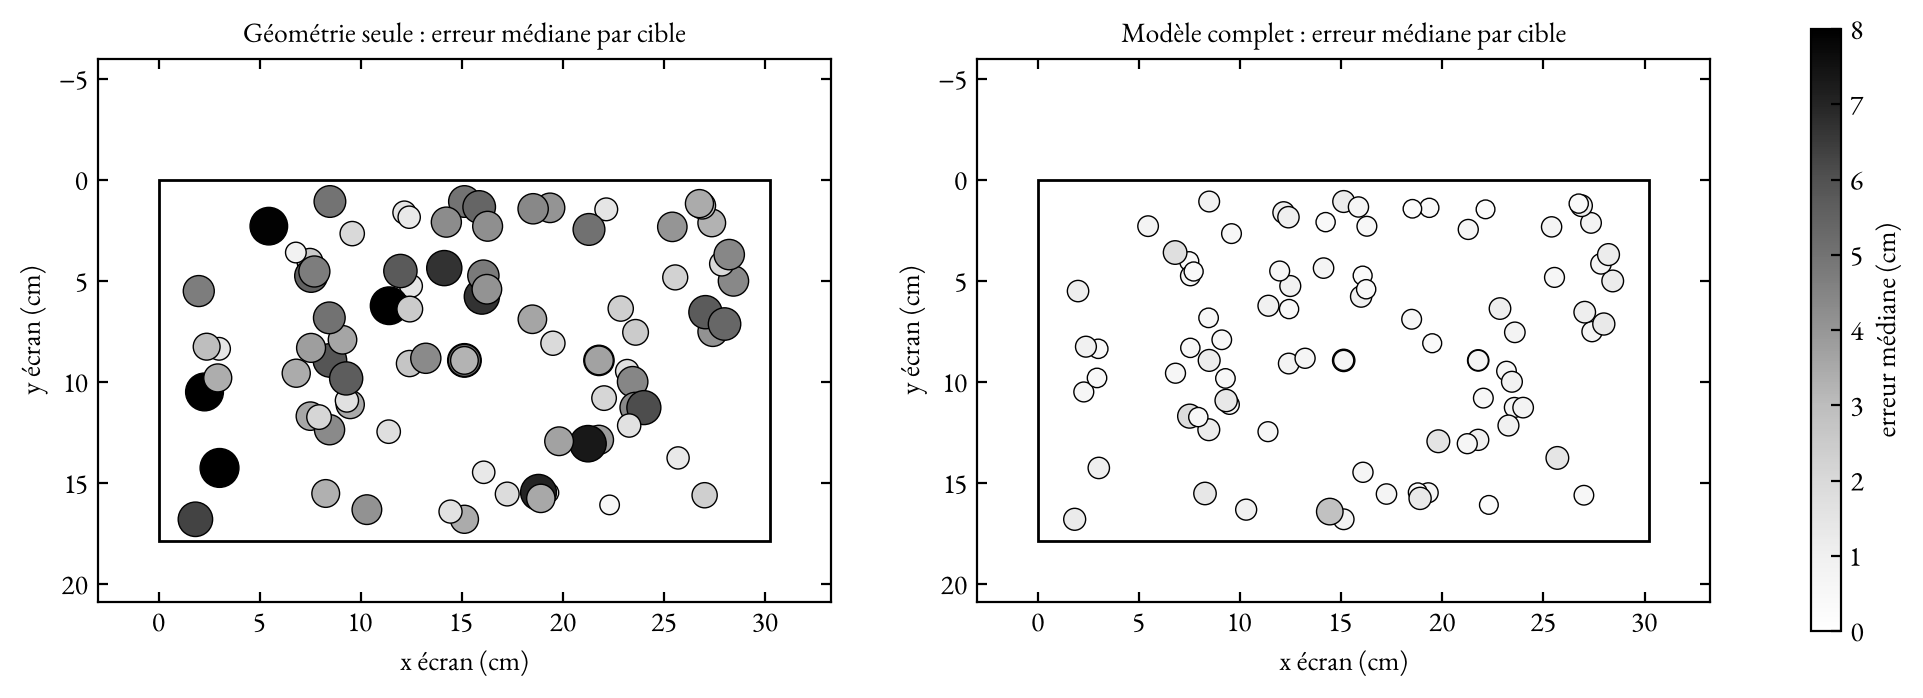
\includegraphics[width=\linewidth]{fig06_erreur_sur_ecran.png}
\caption{Erreur médiane par cible sur l'écran (les points de grille, identiques d'un tour à l'autre, sont regroupés).}\label{fig:carte}
\end{figure}

La vraie difficulté est la posture. Chaque tour occupe une région distincte de l'espace des postures, et donc une région distincte des directions du regard dans la tête (figure~\ref{fig:postures}) : au tour 4, tête levée de 30°, l'œil regarde entre $-20^\circ$ et $-45^\circ$ dans l'orbite, une zone qu'aucun autre tour ne couvre. Tester sur un tour retiré, c'est donc extrapoler. La géométrie seule y souffre partout, de 2,8 à 7,3~cm ; le réseau calibré et le modèle complet restent entre 1,3 et 3,6~cm, le second faisant mieux que le premier sur trois tours sur cinq (figure~\ref{fig:tours}). La recalibration sur cinq points améliore quatre tours sur cinq, jusqu'à 0,7~cm au tour 5, mais dégrade le tour 3, tête tournée de 22° et levée de 12°, de 3,5 à 5,3~cm : les cinq points y sont eux-mêmes mal estimés, et une correction affine à six paramètres ajustée sur cinq points se laisse entraîner par eux.

\begin{figure}[!htbp]
\centering
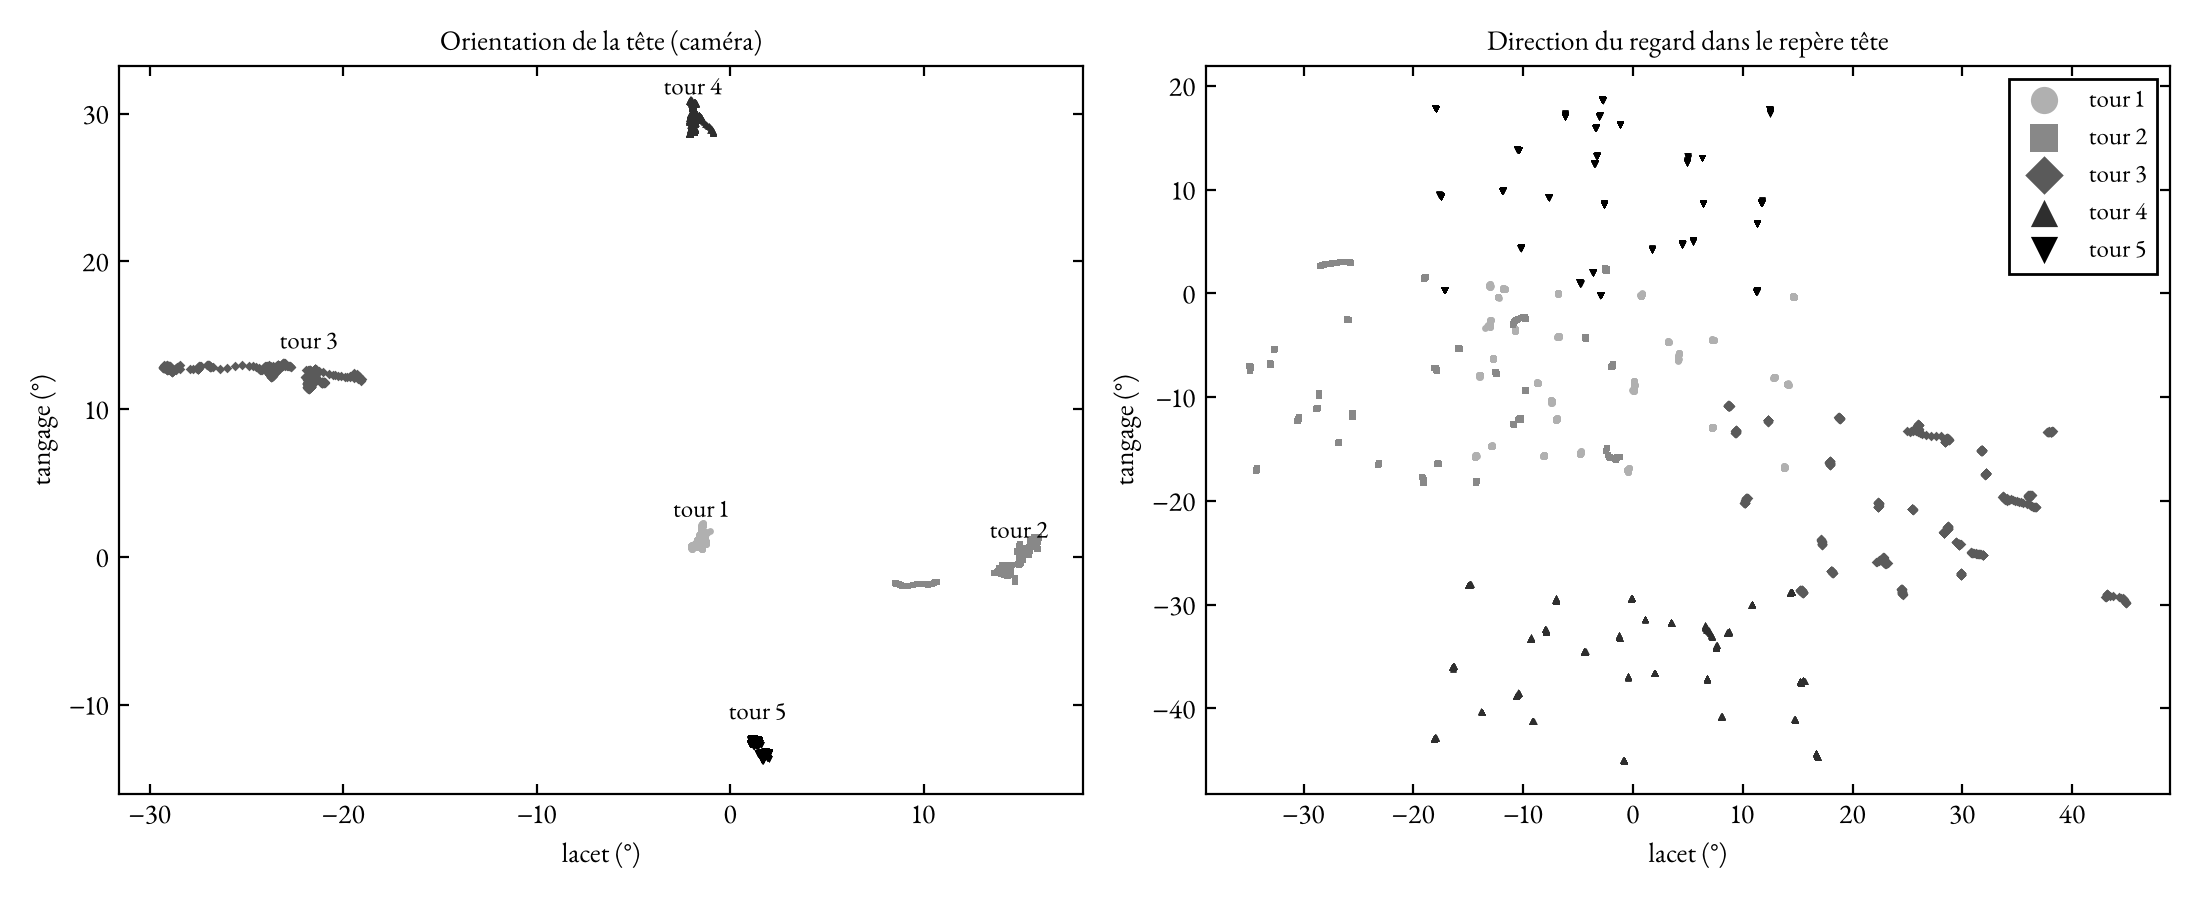
\includegraphics[width=\linewidth]{fig02_postures.png}
\caption{Postures de la tête (à gauche) et directions du regard dans le repère de la tête (à droite), par tour, sur les images de fixation.}\label{fig:postures}
\end{figure}

\begin{figure}[!htbp]
\centering
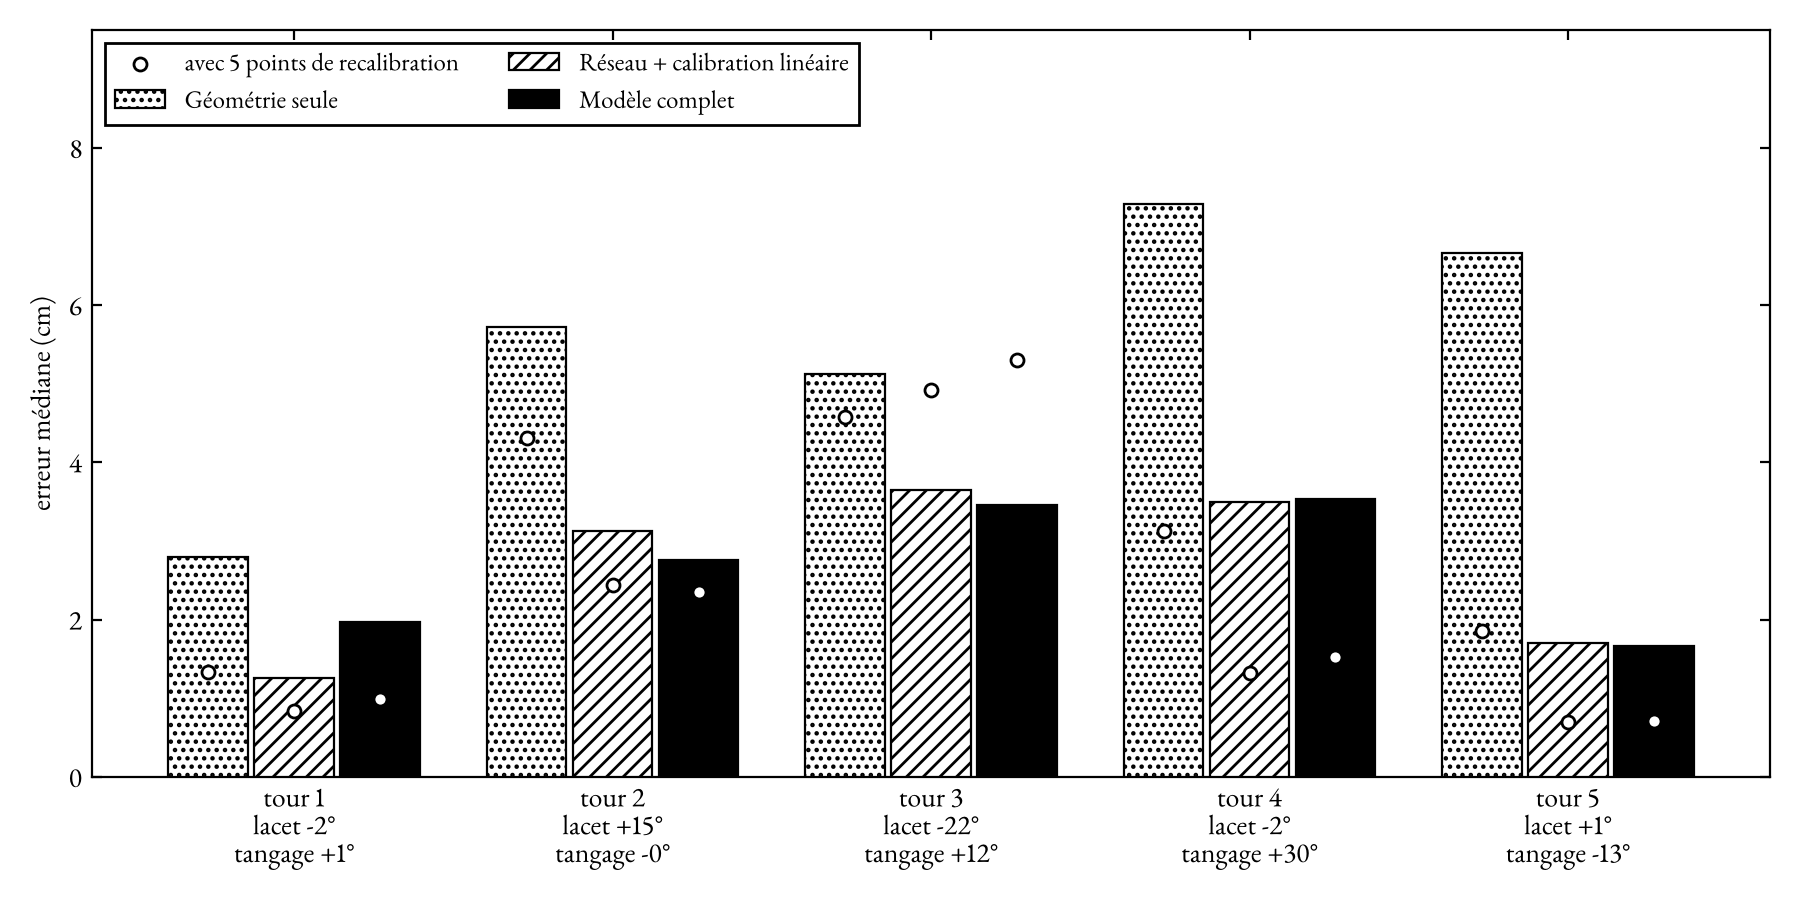
\includegraphics[width=0.85\linewidth]{fig05_posture_jamais_vue.png}
\caption{Posture jamais vue : erreur médiane par tour retiré ; les traits noirs donnent l'erreur après recalibration sur cinq points.}\label{fig:tours}
\end{figure}

\section{Du regard image par image aux fixations}\label{sec:temporal}

Une image est déclarée clignement si les coefficients de clignement des deux yeux dépassent 0,5, et le masque est étendu de $\pm75$~ms. Le regard restant est lissé par le filtre One Euro \cite{casiez2012}, filtre exponentiel dont la fréquence de coupure s'adapte à la vitesse,
\begin{equation}
\hat{\vect x}_n=\hat{\vect x}_{n-1}+a(f_n,\Delta t)\,(\vect x_n-\hat{\vect x}_{n-1}),\qquad
a(f,\Delta t)=\frac{1}{1+\frac{1}{2\pi f\Delta t}},\qquad
f_n=f_{\min}+\beta\,\|\dot{\hat{\vect x}}_n\| ,
\end{equation}
avec $f_{\min}=1$~Hz et $\beta=0{,}3$ : peu de lissage quand l'œil bouge vite, donc pas de retard sur les saccades, beaucoup quand il est fixe, donc pas de tremblement.

Pendant une fixation le regard est constant ; pendant une poursuite il est, localement, affine. On découpe donc la série $\vect z_n=\vect y_n/\vect\sigma$, normalisée par le bruit composante par composante, en segments $[i,j)$ constants ou affines qui minimisent un coût pénalisé,
\begin{equation}
\begin{gathered}
F(n)=\min_{0\le i\le n-m}\Bigl[F(i)+C(i,n)+\lambda\Bigr],\qquad F(0)=0,\\
C(i,j)=\min\bigl(\mathrm{SSE}_0(i,j),\ \mathrm{SSE}_1(i,j)+\lambda_1\bigr),
\end{gathered}
\end{equation}
où $m$ est la durée minimale d'une fixation, 100~ms, $\lambda=3\ln N$ la pénalité par segment, de type BIC, et $\lambda_1=2\lambda$ le surcoût d'une pente. La récurrence est exacte, car tout découpage optimal de $[0,n)$ se termine par un dernier segment $[i,n)$ précédé d'un découpage optimal de $[0,i)$ (principe d'optimalité de Bellman, le coût étant additif sur les segments). Chaque coût se calcule en temps constant à partir des sommes cumulées $S_1,S_t,S_{tt},S_y,S_{yy},S_{ty}$ sur $[i,j)$, calculées une fois pour toutes. Avec $n=S_1$,
\begin{equation}
\mathrm{SSE}_0=\sum(y-\bar y)^2=S_{yy}-\frac{S_y^2}{n}
\end{equation}
(formule de König--Huygens). Pour le modèle affine $y\approx\beta_0+\beta_1t$, les équations normales s'écrivent $\mathbf M\vect\beta=\vect b$ avec $\mathbf M=\begin{psmallmatrix}n&S_t\\S_t&S_{tt}\end{psmallmatrix}$ et $\vect b=(S_y,S_{ty})\T$ ; la somme expliquée est $\vect b\T\mathbf M^{-1}\vect b$ (projection orthogonale sur l'espace engendré par $1$ et $t$), et l'inverse explicite d'une matrice $2\times2$ donne
\begin{equation}
\mathrm{SSE}_1=S_{yy}-\frac{S_{tt}S_y^2-2S_tS_yS_{ty}+n\,S_{ty}^2}{n\,S_{tt}-S_t^2}.
\end{equation}
La récurrence entière coûte ainsi $O(N^2)$, vectorisée sur $i$. Le bruit $\sigma$ s'estime sans se laisser tromper par les mouvements de l'œil : pour un bruit blanc $\varepsilon$ de variance $\sigma^2$, la différence seconde $\varepsilon_{n+1}-2\varepsilon_n+\varepsilon_{n-1}$ a pour variance $(1+4+1)\sigma^2=6\sigma^2$ (variance d'une combinaison linéaire de variables indépendantes), tandis qu'elle annule toute tendance affine. D'où l'estimateur robuste $\hat\sigma=1{,}4826\,\MAD(\Delta^2y)/\sqrt6$, borné inférieurement à $0{,}5^\circ$ parce que MediaPipe lisse déjà ses points et que son erreur réelle est une dérive lente plutôt qu'un bruit blanc. Entre deux segments, enfin, on raccorde par une marche infiniment dérivable, exactement constante avant et après,
\begin{equation}
S(s)=\frac{\phi(s)}{\phi(s)+\phi(1-s)},\qquad\phi(s)=\begin{cases}e^{-1/s}&s>0,\\0&s\le0,\end{cases}
\end{equation}
d'une durée qui suit la séquence principale des saccades \cite{bahill1975}, $T=21~\text{ms}+2{,}2~\text{ms}/^\circ\times A$ pour une amplitude $A$. La fonction $\phi$ est $C^\infty$, toutes ses dérivées tendant vers 0 en $0^+$, et le dénominateur ne s'annule jamais, l'un au moins des deux termes étant strictement positif ; $S$ est donc $C^\infty$, nulle pour $s\le0$ et égale à 1 pour $s\ge1$.

\begin{figure}[!htbp]
\centering
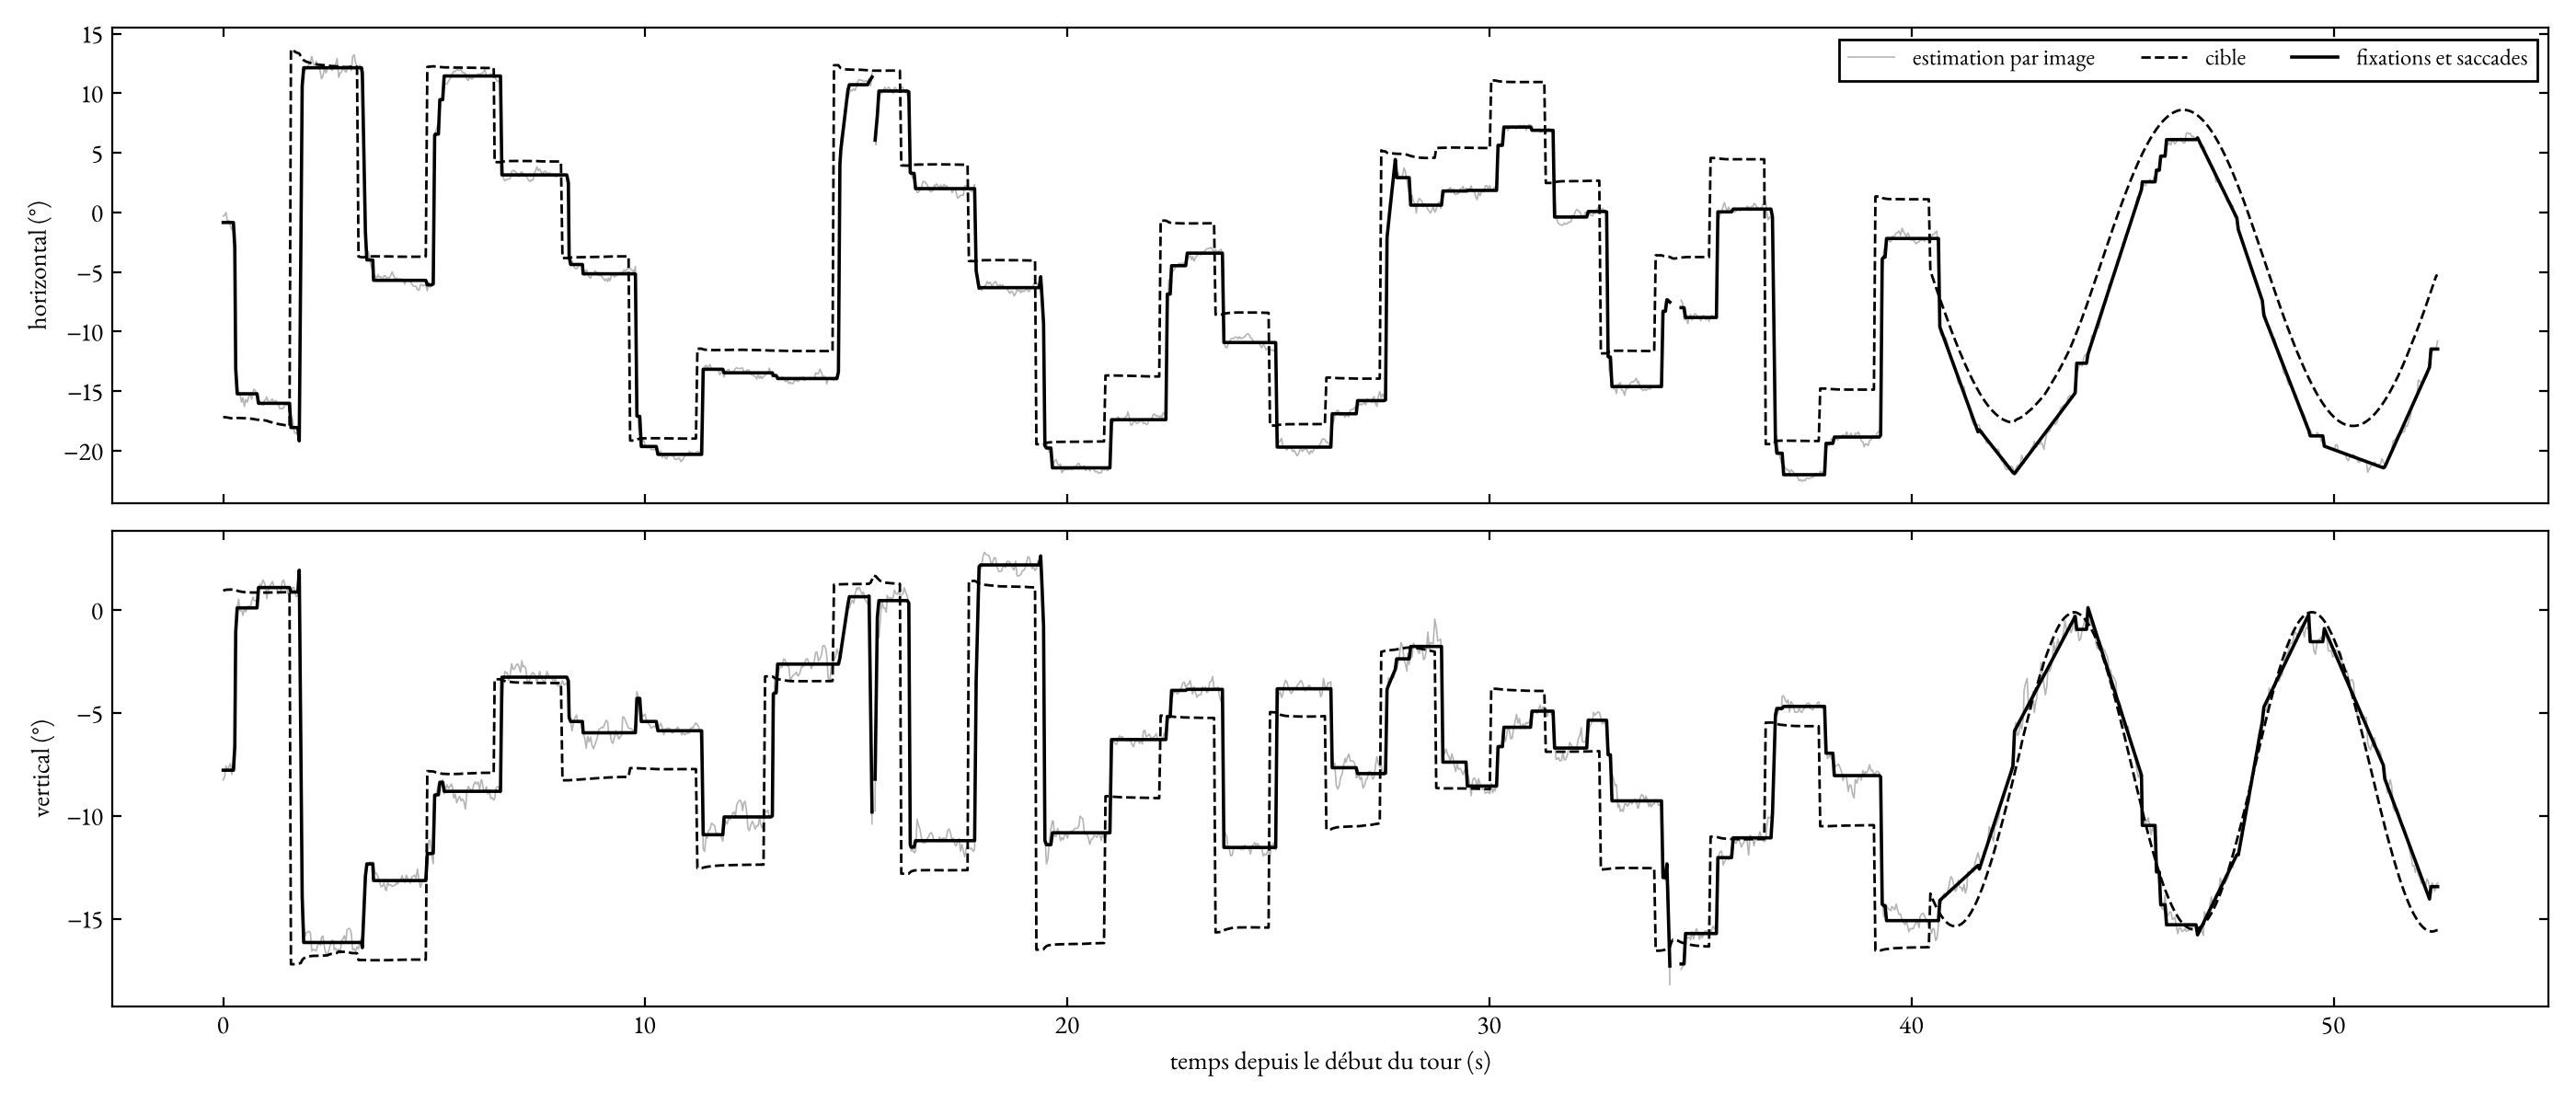
\includegraphics[width=\linewidth]{fig08_serie_temporelle.png}
\caption{Tour 2, prédit sans l'avoir vu : cible (noir), estimation par image (gris) et segmentation en fixations, saccades et poursuite.}\label{fig:serie}
\end{figure}

Sur le tour 2, prédit par un modèle qui ne l'a jamais vu, les marches suivent les sauts de la cible et la poursuite finale est reconnue comme telle (figure~\ref{fig:serie}). Sur l'écran, la poursuite garde sa forme mais se décale d'environ 3~cm (figure~\ref{fig:poursuite}), conséquence de la posture jamais vue et du retard naturel de l'œil sur une cible mobile ; sur les cinq tours, l'erreur médiane en poursuite va de 1,5 à 4,0~cm.

\begin{figure}[!htbp]
\centering
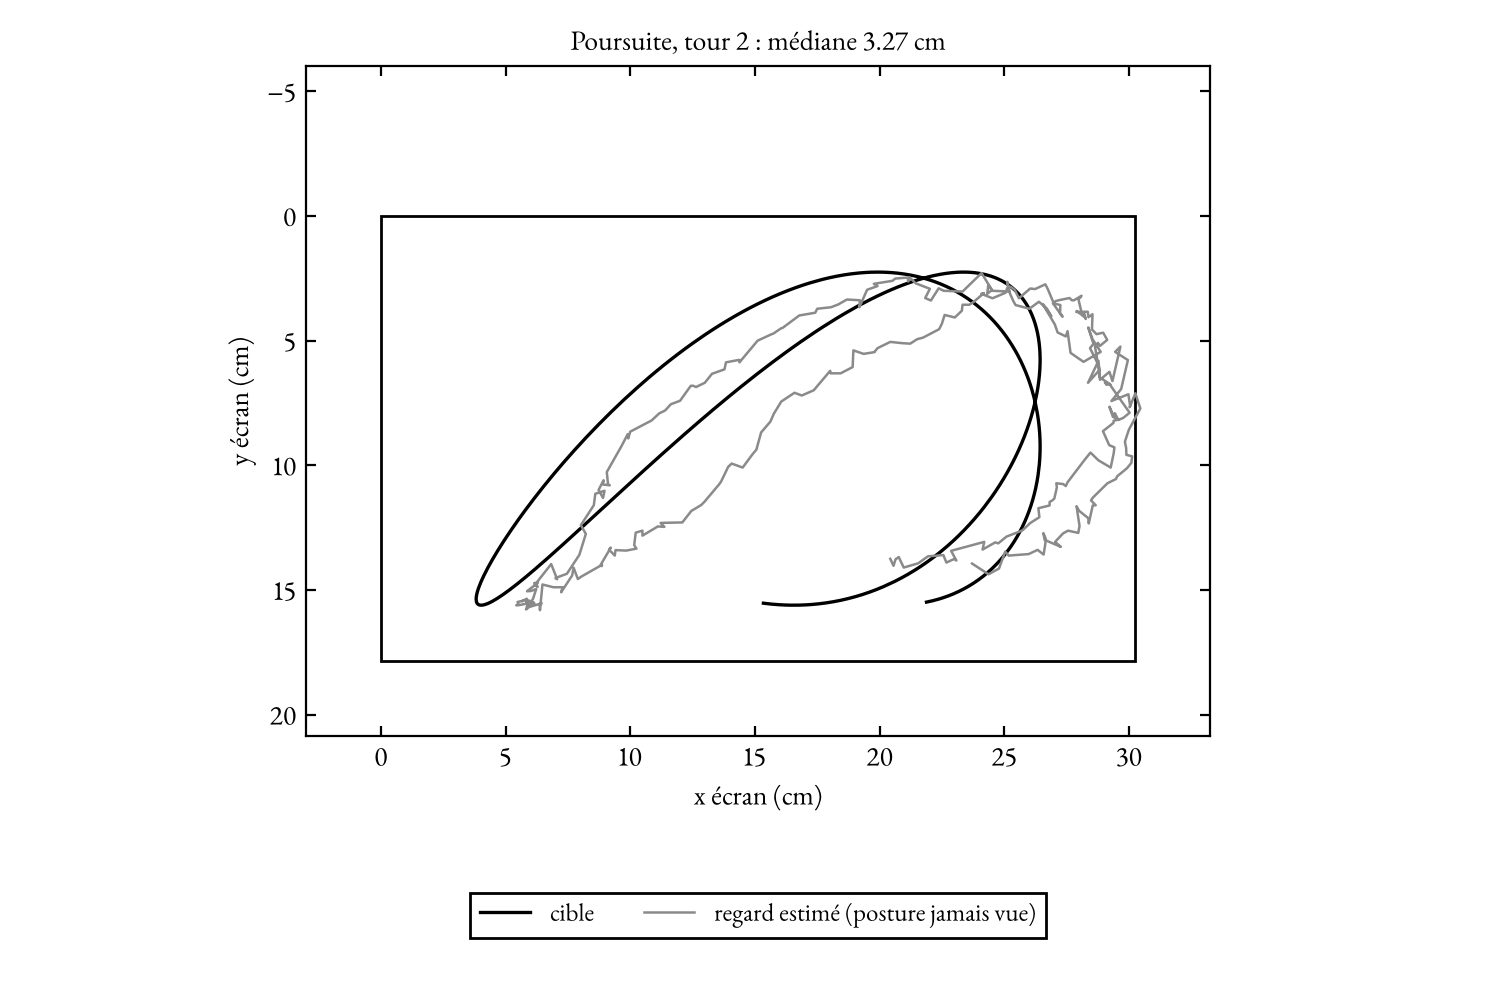
\includegraphics[width=0.6\linewidth]{fig09_poursuite.png}
\caption{Poursuite du tour 2 sur l'écran, tour exclu de l'ajustement.}\label{fig:poursuite}
\end{figure}

\section{Le regard dans le plan complexe}\label{sec:complex}

Une direction de regard est un point de la sphère unité, alors que ce que l'on regarde, un écran, une feuille, un graphique, est un plan. La projection stéréographique fait passer de l'une à l'autre sans rien perdre et transforme la géométrie du regard en calcul sur les nombres complexes. On place l'origine à l'œil cyclope $\vect c$ et l'on prend trois axes liés à la personne, $\vect e_d$ vers sa droite, $\vect e_h$ vers le haut et $\vect e_a$ vers l'avant, perpendiculaire à l'écran ; dans le repère caméra, $\vect e_d=(-1,0,0)$, $\vect e_h=(0,1,0)$ et $\vect e_a=(0,0,1)$, et un vecteur regard unitaire $\vect g$ a pour coordonnées $(u,v,w)=(-g_x,\,g_y,\,g_z)$. On lui associe le nombre complexe
\begin{equation}\label{eq:stereo}
z=\frac{u+i\,v}{1+w},\qquad w>-1,
\end{equation}
qui n'est autre que l'intersection avec le plan $w=0$ de la droite joignant le pôle arrière $\vect S=(0,0,-1)$ au point $(u,v,w)$ : cette droite s'écrit $\vect S+s\bigl((u,v,w)-\vect S\bigr)$, sa troisième coordonnée $-1+s(w+1)$ s'annule pour $s=1/(1+w)$, et le point obtenu est $\bigl(u/(1+w),\,v/(1+w),\,0\bigr)$. Si $\varepsilon$ est l'excentricité du regard, son angle avec $\vect e_a$, et $\psi$ son azimut, alors $(u,v,w)=(\sin\varepsilon\cos\psi,\ \sin\varepsilon\sin\psi,\ \cos\varepsilon)$ et
\begin{align}
z&=\frac{\sin\varepsilon}{1+\cos\varepsilon}\,e^{i\psi}\quad(\text{formule d'Euler})\\
&=\frac{2\sin\frac\varepsilon2\cos\frac\varepsilon2}{2\cos^2\frac\varepsilon2}\,e^{i\psi}\quad(\text{formules de l'angle moitié})\\
&=\tan\frac{\varepsilon}{2}\;e^{i\psi}.
\end{align}
Le module de $z$ dit de combien l'on s'écarte du regard droit devant, son argument dans quelle direction ; la personne regardant droit devant est en $z=0$, et les regards à $10^\circ$, $20^\circ$ et $30^\circ$ forment des cercles concentriques de rayons 0,087, 0,176 et 0,268. Réciproquement, de $|z|^2=\tan^2\frac\varepsilon2=\frac{1-\cos\varepsilon}{1+\cos\varepsilon}$ (angle moitié) on tire $\cos\varepsilon$ par une équation du premier degré, d'où
\begin{equation}
w=\frac{1-|z|^2}{1+|z|^2},\qquad 1+w=\frac{2}{1+|z|^2},\qquad u+iv=z\,(1+w)=\frac{2z}{1+|z|^2}.
\end{equation}
La projection est ainsi une bijection de la sphère privée de $\vect S$ sur $\C$ ; elle est conforme et envoie tout cercle de la sphère ne passant pas par $\vect S$ sur un cercle du plan \cite{needham1997}, de sorte qu'un regard qui décrit un cercle de directions décrit un cercle de $\C$.

Le regard dans le repère caméra est l'orientation de l'œil dans la tête, transportée par la rotation de la tête, $\vect g=\mathbf R\,\vect g_{\text{œil}}$, et dans le repère de la personne la tête agit par $\mathbf R'=\Pi\mathbf R\Pi$, avec $\Pi=\operatorname{diag}(-1,1,1)$, qui est encore une rotation ($\Pi^2=\mathbf I$, $\det\mathbf R'=\det\mathbf R=1$). Soit $(q_0;q_1,q_2,q_3)$ son quaternion unitaire dans les axes $(\vect e_d,\vect e_h,\vect e_a)$. L'action de $\mathbf R'$ sur $z$ est alors l'homographie
\begin{equation}\label{eq:mobius}
M(z)=\frac{a\,z+b}{-\bar b\,z+\bar a},\qquad a=q_0+i\,q_3,\quad b=q_2-i\,q_1,\quad |a|^2+|b|^2=1 .
\end{equation}
Pour le voir, observons d'abord que $q\mapsto\begin{psmallmatrix}a&b\\-\bar b&\bar a\end{psmallmatrix}$ est un morphisme de groupes des quaternions unitaires vers $SU(2)$ (vérification directe sur le produit) et que la composée de deux homographies correspond au produit de leurs matrices ; il suffit donc de vérifier la formule sur des rotations qui engendrent $SO(3)$. Pour une rotation d'angle $\varphi$ autour de $\vect e_a$, $a=e^{i\varphi/2}$ et $b=0$, donc $M(z)=e^{i\varphi}z$, rotation du plan d'angle $\varphi$, ce qui est exactement l'action sur $(u,v)$ à $w$ fixé. Pour une rotation d'angle $\varphi$ autour de $\vect e_h$, qui envoie $\vect e_a$ sur $\sin\varphi\,\vect e_d+\cos\varphi\,\vect e_a$, on a $a=c=\cos\frac\varphi2$ et $b=s=\sin\frac\varphi2$ ; une homographie étant déterminée par les images de trois points, on vérifie $0$, $\infty$ et $1$ :
\begin{align*}
M(0)&=\tfrac{s}{c}=\tan\tfrac\varphi2=\tfrac{\sin\varphi}{1+\cos\varphi}\quad(\text{image de }\vect e_a,\ \text{angle moitié}),\\
M(\infty)&=-\tfrac{c}{s}=-\tfrac{\sin\varphi}{1-\cos\varphi}\quad(\text{image de }\vect S=(-\sin\varphi,0,-\cos\varphi)),\\
M(1)&=\tfrac{c+s}{c-s}=\tfrac{(c+s)^2}{c^2-s^2}=\tfrac{1+\sin\varphi}{\cos\varphi}=\tfrac{\cos\varphi}{1-\sin\varphi}\quad(\text{image de }\vect e_d=(\cos\varphi,0,-\sin\varphi)).
\end{align*}
Toute rotation étant un produit de rotations autour de $\vect e_a$ et de $\vect e_h$ (angles d'Euler), la formule \eqref{eq:mobius} vaut pour toute rotation. Le regard se décompose donc exactement en tête et œil,
\begin{equation}
z_{\text{regard}}=M_{\text{tête}}\bigl(z_{\text{œil}}\bigr),\qquad z_{\text{tête}}=M_{\text{tête}}(0),
\end{equation}
où $z_{\text{tête}}$ est la direction de la normale du visage. Pour une tête presque de face, $b$ et $q_3$ sont petits ; au premier ordre $M_{\text{tête}}(z)\approx z+b+2iq_3z$ et $z_{\text{tête}}\approx b$, d'où
\begin{equation}
z_{\text{regard}}\approx z_{\text{tête}}+z_{\text{œil}}+2iq_3\,z_{\text{œil}} :
\end{equation}
les directions s'additionnent comme des nombres complexes, à un terme de roulis près. Sur la séance, la composition exacte reproduit le regard à $1{,}5\cdot10^{-7}$ près, l'écart venant de l'arrondi en simple précision des matrices de pose.

L'écran est le plan perpendiculaire à $\vect e_a$ situé à la distance $D=-c_z$ devant l'œil. Le rayon $\vect c+s\vect g$ l'atteint pour $s=D/w$, au point décalé de $D\,(u+iv)/w$ par rapport au pied de la perpendiculaire, et les formules inverses donnent
\begin{equation}
\Phi(z)=D\,\frac{u+iv}{w}=D\,\frac{2z/(1+|z|^2)}{(1-|z|^2)/(1+|z|^2)}=\frac{2D\,z}{1-|z|^2}.
\end{equation}
L'écran est donc l'image du disque unité par $\Phi$, et près du centre $\Phi(z)\approx2Dz$ : à $10^\circ$ d'excentricité, l'écart relatif $|z|^2/(1-|z|^2)$ reste sous 0,8\,\%. À 52~cm, un centième de $|z|$ vaut 1,04~cm sur l'écran ; le plan complexe est l'écran vu depuis l'œil, à l'échelle $2D$ (figure~\ref{fig:complexe}).

\begin{figure}[!htbp]
\centering
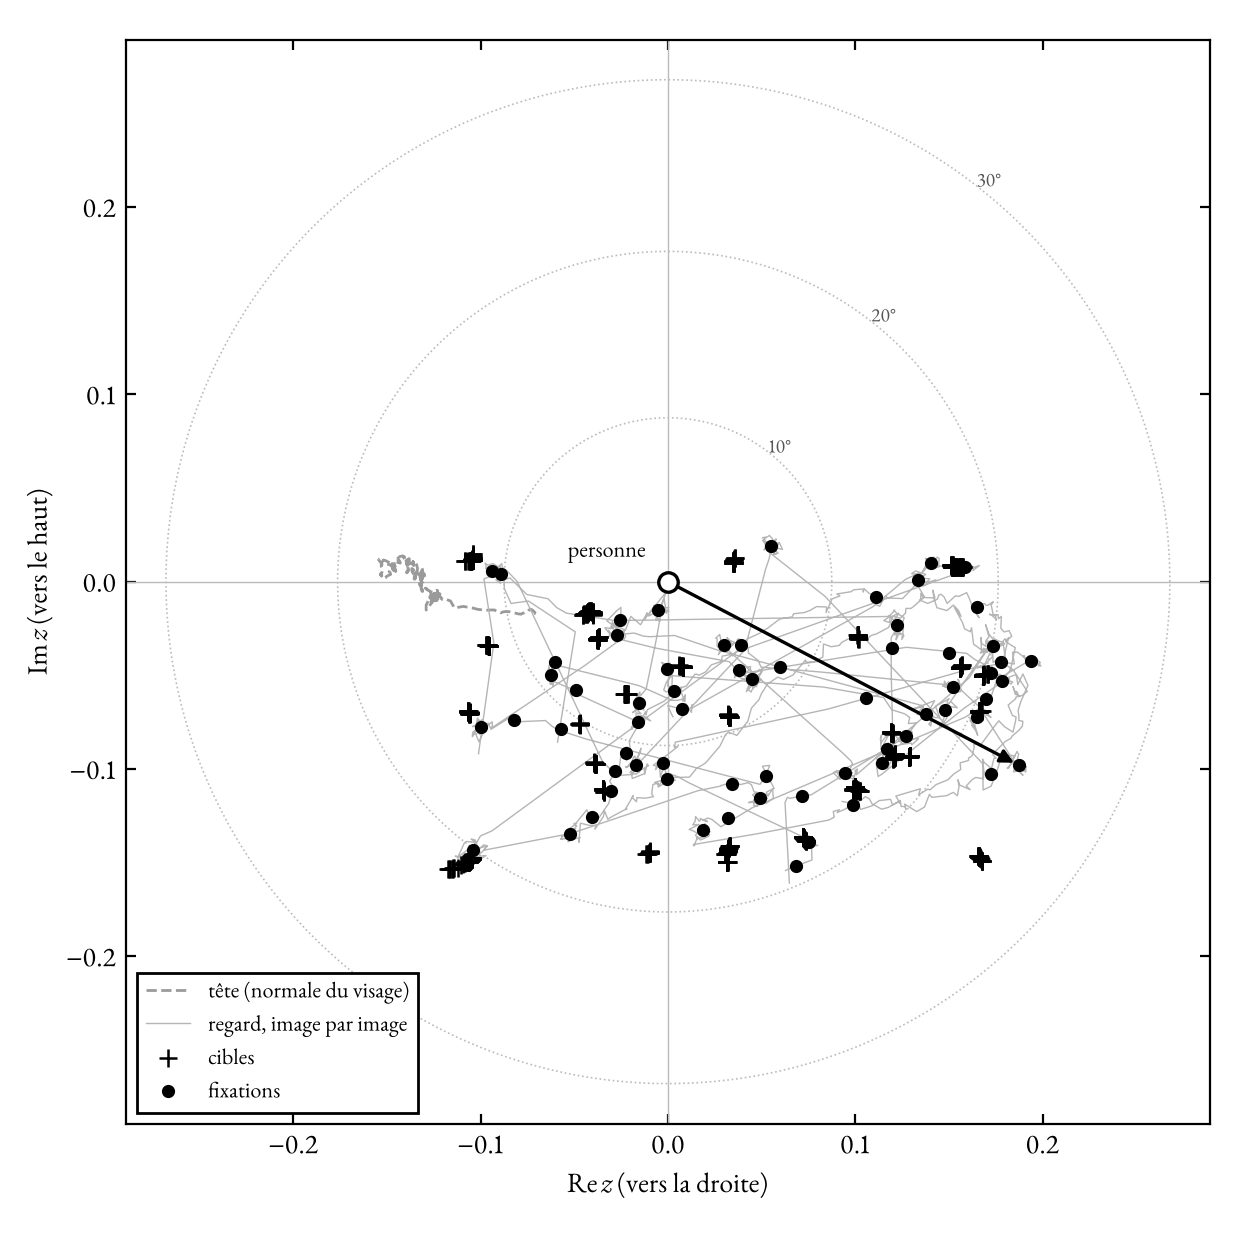
\includegraphics[width=0.72\textwidth]{fig11_plan_complexe.png}
\caption{Le tour 2 dans le plan complexe, prédit par un modèle qui n'a jamais vu ce tour. La personne est en $0$ ; les cercles pointillés sont les excentricités de $10^\circ$, $20^\circ$ et $30^\circ$. Disques : fixations détectées ; croix : cibles ; tirets : direction de la tête $z_{\text{tête}}$ ; la flèche est le vecteur regard de la fixation la plus excentrée.}\label{fig:complexe}
\end{figure}

Au fil du temps, enfin, $z(t)$ décrit une courbe de $\R\times\C\simeq\R^3$,
\begin{equation}
\Gamma=\bigl\{\,(t,\ \operatorname{Re}z(t),\ \operatorname{Im}z(t))\ :\ t\in[0,T]\,\bigr\},
\end{equation}
dont l'axe $\{z=0\}$ est la personne regardant droit devant ; à chaque instant, le vecteur regard est le segment qui joint $(t,0)$ à $(t,z(t))$. Les trois régimes de l'œil y prennent trois formes simples. Une fixation, $z$ constant sur $[t_1,t_2]$, est un segment parallèle à l'axe du temps. Une saccade est un saut de durée $T=21~\text{ms}+2{,}2~\text{ms}/^\circ\times A$, presque perpendiculaire à cet axe. Une poursuite d'une cible qui tourne à excentricité constante $\varepsilon_0$ et à vitesse angulaire $\omega$ donne $z(t)=\tan\frac{\varepsilon_0}{2}\,e^{i(\omega t+\psi_0)}$, hélice de rayon $\tan\frac{\varepsilon_0}{2}$ et de pas $2\pi/\omega$, l'arc de cercle déroulé dans le temps. La poursuite de la calibration suit une courbe de Lissajous, qui devient dans $\Gamma$ la succession d'arcs de la figure~\ref{fig:trajectoire}.

\begin{figure}[!htbp]
\centering
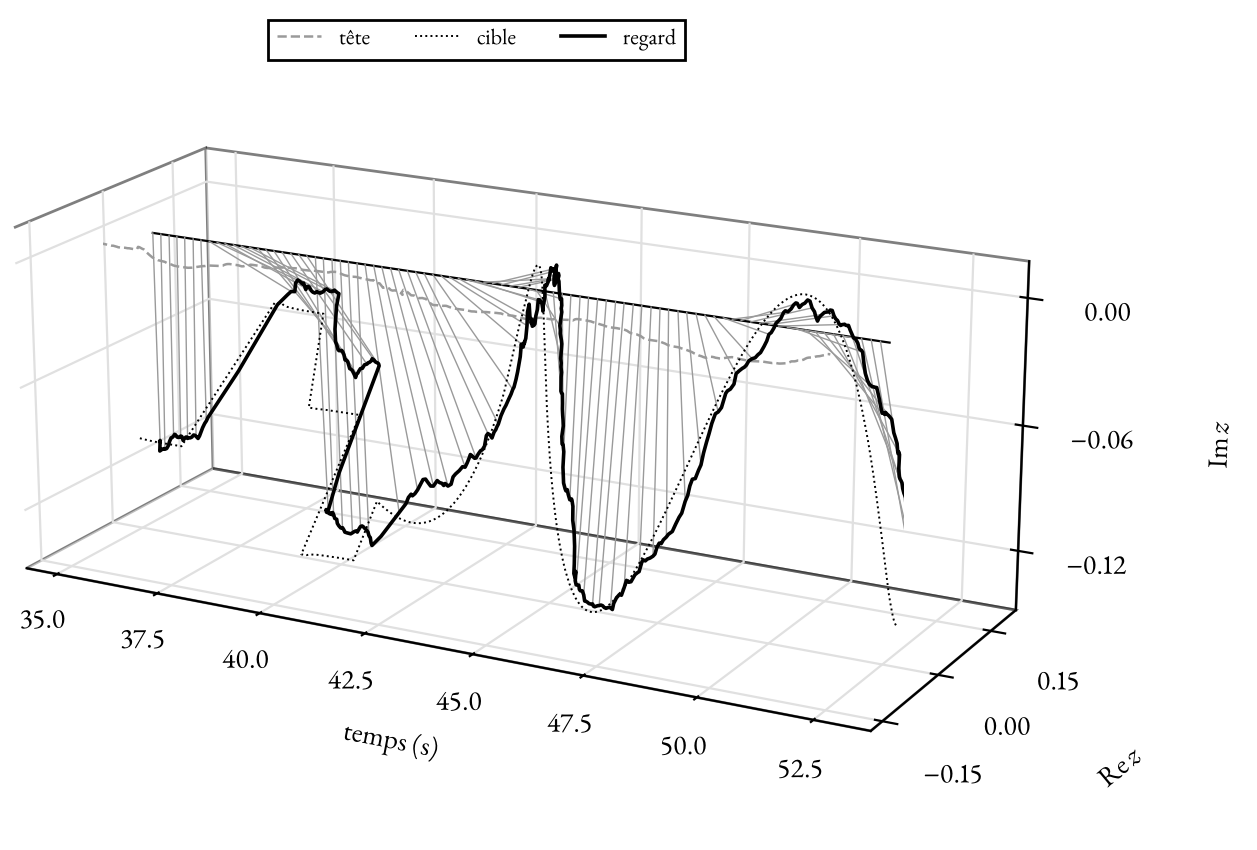
\includegraphics[width=\textwidth]{fig12_trajectoire_complexe.png}
\caption{Trajectoire du regard dans $\R\times\C$ sur les 17 dernières secondes du tour 2 : quelques fixations, paliers parallèles à l'axe du temps, puis la poursuite, en arcs. L'axe noir est la personne ($z=0$), chaque trait gris le vecteur regard à un instant ; pointillés : la cible ; tirets : la tête.}\label{fig:trajectoire}
\end{figure}

\section{Complexité et temps de calcul}\label{sec:complexity}

Notons $N$ le nombre d'images, $N_c\approx4\,000$ le nombre d'images de calibration, $p=8$ le nombre de paramètres physiques, $I$ le nombre d'itérations, $F$ le nombre de décalages testés pour la synchronisation et $P$ le nombre de plis. L'extraction est parallélisée par morceaux de vidéo et sauvegardée toutes les 500 images, la validation sauvegarde chaque pli, et un calcul interrompu reprend où il s'était arrêté (tableau~\ref{tab:complexite}).

\begin{table}[!htbp]
\centering\footnotesize
\begin{tabular}{@{}p{3.3cm}p{4.4cm}p{3.4cm}@{}}
\toprule
Étape & Complexité & Mesure (CPU, cette séance)\\
\midrule
Points MediaPipe & $O(N)$ & $\approx25$ images/s par cœur\\
Réseaux (normalisation + 2 ResNet) & $O(N)$ & $\approx7$ images/s par cœur\\
Imagettes des yeux & $O(N)$ & 1~min\\
Synchronisation & $O(NF)$ & quelques secondes\\
Modèle physique & $O(I\,N_c\,p)$ & quelques secondes\\
Étage linéaire & $O(N_c)$ & négligeable\\
Régression à noyau & $O(N_c^3)$ ajustement, $O(N\,N_c)$ prédiction & quelques secondes par pli\\
Validation complète & $O(P\,N_c^3)$, $P=10$ & moins d'une minute\\
Segmentation & $O(N^2)$ par bloc continu & quelques secondes\\
Plan complexe & $O(N)$ & négligeable\\
\bottomrule
\end{tabular}
\caption{Complexité temporelle des étapes.}\label{tab:complexite}
\end{table}

\section{Discussion}\label{sec:discussion}

Que vaut une erreur de 0,88° ? La fovéola, la petite zone de la rétine où la vision est la plus nette, couvre environ un degré du champ visuel, et l'œil lui-même, pendant une fixation, dérive et tremble de quelques dixièmes de degré. Dans la zone calibrée, le système désigne donc la région que la personne voit nettement ; les eye trackers infrarouges du commerce, avec leur éclairage et leur caméra dédiés, annoncent environ un demi-degré. L'erreur n'est pas nulle et ne peut pas l'être. Une part en revient à la vérité terrain, puisque la cible n'est pas exactement le point fixé ; une part au bruit des points de MediaPipe, qui est de l'ordre du pixel sur un iris de vingt pixels de diamètre ; une part, enfin, au modèle. Les essais faits pour réduire cette dernière disent où se trouve la marge : élargir l'embedding des réseaux à 32 ou 64 composantes dégrade le résultat, doubler le nombre de composantes des imagettes ne change rien, et c'est l'ajout des pixels des yeux, non celui de paramètres, qui a fait passer l'erreur par fixation de 0,71 à 0,66~cm. Le modèle est désormais limité par l'information que contient l'image plus que par sa propre capacité.

La posture est l'autre limite, et la plus sérieuse : hors de la zone calibrée, l'erreur remonte à 2,7~cm. La structure en deux étages garantit que cette dégradation reste douce \eqref{eq:extrapolation}, mais elle ne crée pas l'information manquante, et une calibration qui couvre les postures réellement utilisées reste la meilleure parade. Les chiffres viennent en outre d'une seule personne et d'une seule séance : la généralisation entre personnes reste à mesurer, et les hyperparamètres, nombres de composantes et régularisation, ont été choisis parmi une vingtaine de variantes sur ces mêmes plis, ce qui laisse attendre sur une nouvelle séance une erreur plus élevée de 0,1 à 0,2~cm. Les poids des réseaux, enfin, sont entraînés sur des données sous licence non commerciale, et le traitement, hors ligne, est limité par eux à environ sept images par seconde et par cœur.

\section{Conclusion}

L'algorithme tient finalement en une phrase : on détecte les yeux, on y lit la pupille par le centre du limbe, on compose l'orientation de la tête et celle de l'œil pour obtenir le vecteur regard, et l'on suit ce vecteur, devenu un nombre complexe, à travers le temps. Aucune des briques ne suffit seule. La géométrie extrapole mais reste grossière ; les réseaux publics sont robustes mais biaisés ; une correction apprise sur nos seules données serait précise mais aveugle hors de sa zone. Réunies, elles se complètent : la géométrie donne le cadre et l'échelle, le réseau la direction, l'étage linéaire garantit l'extrapolation, et la régression à noyau ajoute la précision là où elle est permise en s'effaçant d'elle-même ailleurs. Le plan complexe, de son côté, transforme la composition de la tête et de l'œil en produit d'homographies, l'écran en image conforme du disque, et la dynamique de l'œil en une courbe où fixations, saccades et poursuites se lisent à l'œil nu. La suite naturelle est une calibration guidée qui couvre d'elle-même les postures manquantes, puis la généralisation à plusieurs personnes et le temps réel, en distillant les deux réseaux en un seul modèle léger.

\section*{Reproductibilité}

Depuis la racine du dépôt, les deux commandes
\begin{verbatim}
python code/calibrate.py \
    data/calibration/calib_20261025_102754.mp4 \
    --log data/calibration/calib_20261025_102754.json
python code/make_results.py
\end{verbatim}
extraient les points, les sorties des réseaux et les imagettes, exécutent les dix plis de validation, ajustent le modèle final et régénèrent toutes les figures et tous les tableaux de cet article, la seconde relisant la vidéo pour la figure~\ref{fig:detection}. Le programme \texttt{code/track.py} applique l'algorithme à n'importe quelle vidéo et écrit, pour chaque image, le vecteur regard, sa décomposition en tête et œil, le nombre complexe $z$ et les fixations.

\begin{thebibliography}{99}
\bibitem{bahill1975} A.~T. Bahill, M.~R. Clark, L.~Stark. The main sequence, a tool for studying human eye movements. \emph{Mathematical Biosciences}, 24(3--4):191--204, 1975.
\bibitem{casiez2012} G.~Casiez, N.~Roussel, D.~Vogel. 1\,€ filter: a simple speed-based low-pass filter for noisy input in interactive systems. \emph{CHI}, 2012.
\bibitem{hysts} hysts. \texttt{pytorch\_mpiigaze\_demo} (ptgaze), \url{https://github.com/hysts/pytorch_mpiigaze_demo}.
\bibitem{kartynnik2019} Y.~Kartynnik, A.~Ablavatski, I.~Grishchenko, M.~Grundmann. Real-time facial surface geometry from monocular video on mobile GPUs. \emph{CVPR Workshops}, 2019.
\bibitem{krafka2016} K.~Krafka, A.~Khosla, P.~Kellnhofer, H.~Kannan, S.~Bhandarkar, W.~Matusik, A.~Torralba. Eye tracking for everyone. \emph{CVPR}, 2016.
\bibitem{needham1997} T.~Needham. \emph{Visual Complex Analysis}. Oxford University Press, 1997.
\bibitem{scholkopf2001representer} B.~Schölkopf, R.~Herbrich, A.~J. Smola. A generalized representer theorem. \emph{COLT}, 2001.
\bibitem{zhang2017mpiifacegaze} X.~Zhang, Y.~Sugano, M.~Fritz, A.~Bulling. It's written all over your face: full-face appearance-based gaze estimation. \emph{CVPR Workshops}, 2017.
\bibitem{zhang2018revisiting} X.~Zhang, Y.~Sugano, A.~Bulling. Revisiting data normalization for appearance-based gaze estimation. \emph{ETRA}, 2018.
\bibitem{zhang2020eth} X.~Zhang, S.~Park, T.~Beeler, D.~Bradley, S.~Tang, O.~Hilliges. ETH-XGaze: a large scale dataset for gaze estimation under extreme head pose and gaze variation. \emph{ECCV}, 2020.
\end{thebibliography}

\end{document}
